% ----------------------------------------------------------------------------
%
%                           Probability and Statistics
%                                  Cookbook
%
% ----------------------------------------------------------------------------
%
% Copyright © Matthias Vallentin <vallentin@icir.org>, 2014
%

\documentclass[landscape]{article}

\usepackage{array}
\usepackage{amsmath,amssymb}
\usepackage{booktabs}
\usepackage{caption}
\usepackage[nodayofweek]{datetime}
\usepackage{environ}
\usepackage{float}
\usepackage{enumitem}
\usepackage{fancyhdr}
\usepackage[landscape,margin=13mm,footskip=1pt,includefoot]{geometry}
\usepackage{graphicx}
\usepackage{hyperref}
\usepackage{multicol}
\usepackage{rotating}
\usepackage{tikz}
\usepackage{translator}
\usepackage{url}
\usepackage{xspace}

% Alias for \translate.
\newcommand{\T}[1]{\translate{#1}}

% Language configuration.
\input{./config}
\usedictionary{probstat}

% Probability and Statistics LaTeX shortcuts. (Not part of the repository.)
\usepackage{amsmath,amssymb}
\usepackage{dsfont}
\usepackage{cancel}
\usepackage{graphicx}
\usepackage{xargs}
\usepackage{xspace}

% =============================================================================
%                                  Formatting
% =============================================================================

% Make a note on the margin.
\newcommand{\marnote}[1]{
  \reversemarginpar
  \marginpar[\raggedleft\footnotesize\textit{\\[3ex]#1}]%
      {\raggedright\footnotesize\textit{\\[3ex]#1}}
  \normalmarginpar
}

\newcommand{\pwiseii}[1]{\ensuremath{\left\{\begin{array}{ll}#1\end{array}}}
\newcommand{\pwiseiii}[1]{\ensuremath{\left\{\begin{array}{ll}#1\end{array}}}
\newcommand{\prn}[1]{\ensuremath{\left(#1\right)}}
\newcommand{\brk}[1]{\ensuremath{\left[#1\right]}}
\newcommand{\brc}[1]{\ensuremath{\left\{#1\right\}}}
\newcommand{\x}[1]{\ensuremath{\cancel{#1}}}

% =============================================================================
%                                 General Math
% =============================================================================

% Special functions and operators
\DeclareMathOperator{\erf}{erf}
\DeclareMathOperator{\logit}{logit}
\DeclareMathOperator{\sign}{sign}
\DeclareMathOperator*{\argmin}{\arg\!\min}

% Definitions
\def\define{:=}
\def\defined{=:}
\def\eqdef{\triangleq}

% Proofs
\def\qed{\ifhmode\unskip\nobreak\fi\hfill \ensuremath{\square}}

% Standard transformation function
\def\transform{\ensuremath{\varphi}\xspace}

% Logic
\newcommand{\comp}[1]{\neg{#1}}
\newcommand{\imp}{\ensuremath{\;\Longrightarrow\;}}
\newcommand{\pmi}{\ensuremath{\;\Longleftarrow\;}}
\newcommand{\nimp}{\ensuremath{\;\not\!\!\Longrightarrow\;}}
\newcommand{\npmi}{\ensuremath{\;\not\!\!\Longleftarrow\;}}
\newcommand{\eqv}{\ensuremath{\;\Longleftrightarrow\;}}

% Numbers.
\def\C{\mathbb{C}}
\def\N{\mathbb{N}}
\def\R{\mathbb{R}}
\def\Z{\mathbb{Z}}

% Matrices
\newcommand{\eyeii}{\ensuremath{\left(\begin{matrix}1 & 0 \\ 0 & 1\end{matrix}\right)}}
\newcommand{\eyeiii}{\ensuremath{\left(\begin{matrix}1 & 0 & 0 \\ 0 & 1 & 0 \\ 0 & 0 & 1\end{matrix}\right)}}

% Limits
\newcommand{\Lim}[2]{\ensuremath{\lim_{#1\to #2}}}
\newcommand{\limx}[1][\infty]{\ensuremath{\lim_{x\to #1}}}
\newcommand{\limn}[1][\infty]{\ensuremath{\lim_{n\to #1}}}

% Sums and products
\newcommand{\Sum}[2][i=1]{\ensuremath{\sum_{#1}^{#2}}}
\newcommand{\sumin}{\ensuremath{\sum_{i=1}^n}}
\newcommand{\sumiN}{\ensuremath{\sum_{i=1}^N}}
\newcommand{\sumim}{\ensuremath{\sum_{i=1}^m}}
\newcommand{\sumjk}{\ensuremath{\sum_{j=1}^k}}
\newcommand{\sumjn}{\ensuremath{\sum_{j=1}^n}}
\newcommand{\sumjm}{\ensuremath{\sum_{j=1}^m}}
\newcommand{\isum}[1][n]{\ensuremath{\sum_{#1}^\infty}}
\newcommand{\dsum}[4][i=1]{\ensuremath{\sum_{#1}^{#2}\sum_{#3}^{#4}}}
\newcommand{\Prod}[2][i=1]{\ensuremath{\prod_{#1}^{#2}}}
\newcommand{\prodin}{\ensuremath{\prod_{i=1}^n}}
\newcommand{\prodjn}{\ensuremath{\prod_{j=1}^n}}

% Derivatives
\newcommand{\der}[2][]{\ensuremath{\frac{d #1}{d #2}}}
\newcommand{\dder}[2][]{\ensuremath{\frac{d^2 #1}{d #2^2}}}
\newcommand{\pder}[2][]{\ensuremath{\frac{\partial #1}{\partial #2}}}
\newcommand{\pdder}[2][]{\ensuremath{\frac{\partial^2 #1}{\partial #2^2}}}
\newcommand{\mpder}[3][]{%
  \ensuremath{\frac{\partial^2 #1}{\partial #2 \partial #3}}}

% Differentials
%\renewcommand{\d}[1]{\,\mathrm{d}#1}
\renewcommand{\d}[1]{\,d#1}
\def\ds{\d{s}}
\def\dt{\d{t}}
\def\dtheta{\d{\theta}}
\def\du{\d{u}}
\def\dx{\d{x}}
\def\dy{\d{y}}
\def\dfx{\d{F_X(x)}}
\def\dfy{\d{F_Y(y)}}
\def\dfhatx{\d{\widehat{F}_n(x)}}

% Transcendentals w/ extended arguments.
\newcommand{\Exp}[1]{\ensuremath{\exp\left\{#1\right\}}}
\newcommand{\Log}[1]{\ensuremath{\log\left\{#1\right\}}}

% =============================================================================
%                          Probability and Statistics
% =============================================================================

% Formatted terminology.
\def\bias{\textsf{bias}\xspace}
\def\se{\textsf{se}\xspace}
\def\pdf{\textsc{pdf}\xspace}
\def\cdf{\textsc{cdf}\xspace}
\def\ise{\textsc{ise}\xspace}
\def\pgf{\textsc{pgf}\xspace}
\def\mgf{\textsc{mgf}\xspace}
\def\mse{\textsc{mse}\xspace}
\def\mspe{\textsc{mspe}\xspace}
\def\mle{\textsc{mle}\xspace}
\def\mom{\textsc{mom}\xspace}
\def\are{\textsc{are}\xspace}
\def\rss{\textsc{rss}\xspace}
\def\ess{\textsc{ess}\xspace}
\def\tss{\textsc{tss}\xspace}

% Naming shortcuts.
\def\ahat{\ensuremath{\widehat{\alpha}}}
\def\atil{\ensuremath{\tilde{\alpha}}}
\def\bhat{\ensuremath{\widehat{\beta}}}
\def\btil{\ensuremath{\tilde{\beta}}}
\def\dhat{\ensuremath{\widehat{\delta}}}
\def\ehat{\ensuremath{\hat{\epsilon}}}
\def\ghat{\ensuremath{\widehat{\gamma}}}
\def\khat{\ensuremath{\widehat{\kappa}}}
\def\lhat{\ensuremath{\widehat{\lambda}}}
\def\ltil{\ensuremath{\tilde{\lambda}}}
\def\mhat{\ensuremath{\widehat{\mu}}}
\def\nhat{\ensuremath{\widehat{\nu}}}
\def\mtil{\ensuremath{\tilde{\mu}}}
\def\psihat{\ensuremath{\widehat{\psi}}}
\def\shat{\ensuremath{\widehat{\sigma}}}
\def\stil{\ensuremath{\tilde{\sigma}}}
\def\that{\ensuremath{\widehat{\theta}}}
\def\ttil{\ensuremath{\widetilde{\theta}}}
\def\rhohat{\widehat{\rho}}
\def\xihat{\widehat{\xi}}

\def\sehat{\ensuremath{\widehat{\se}}}
\def\fhat{\ensuremath{\widehat{f}}}
\def\Fhat{\ensuremath{\widehat{F}}}
\def\fnhat{\ensuremath{\widehat{f}_n}}
\def\Fnhat{\ensuremath{\widehat{F}_n}}
\def\Jhat{\ensuremath{\widehat{J}}}
\def\phat{\ensuremath{\widehat{p}}}
\def\ptil{\ensuremath{\tilde{p}}}
\def\rhat{\widehat{r}}
\def\Rbar{\bar{R}}
\def\Rhat{\widehat{R}}
\def\Qbar{\bar{Q}}
\def\Qhat{\widehat{Q}}
\def\Xhat{\widehat{X}}
\def\xbar{\bar{x}}
\def\Xbar{\bar{X}}
\def\Xsqbar{\overline{X^2}}
\def\xnbar{\overline{x}_n}
\def\Xnbar{\overline{X}_n}
\def\Yhat{\widehat{Y}}
\def\ybar{\overline{y}}
\def\Ybar{\overline{Y}}
\def\Ynbar{\overline{Y}_n}

% Random variables.
\def\rv{\textsc{rv}\xspace}
\def\iid{\ensuremath{\textsc{iid}}\xspace}
\def\dist{\ensuremath{\sim}\xspace}
\def\disteq{\ensuremath{\stackrel{D}{=}}\xspace}
\def\distiid{\ensuremath{\stackrel{iid}{\sim}}\xspace}
\def\ind{\ensuremath{\perp\!\!\!\perp}\xspace}
\def\nind{\ensuremath{\perp\!\!\!\!\big\vert\!\!\!\!\perp}\xspace}
\def\Xon{\ensuremath{X_1,\dots,X_n}\xspace}
\def\xon{\ensuremath{x_1,\dots,x_n}\xspace}
\def\giv{\ensuremath{\,|\,}}
\def\Giv{\ensuremath{\,\big|\,}}
\def\GIV{\ensuremath{\,\Big|\,}}
\newcommand{\indicator}[1]{\mathds{1}_{\left\{#1\right\}}}

% Probability, expectation, and variance.
\def\prob{\mathbb{P}}
\renewcommand{\Pr}[2][]{\ensuremath{\prob_{#1}\left[#2\right]}\xspace}
\newcommand{\E}[2][]{\ensuremath{\mathbb{E}_{#1}\left[#2\right]}}
\newcommand{\V}[2][]{\ensuremath{\mathbb{V}_{#1}\left[#2\right]}}
\newcommand{\cov}[2][]{\ensuremath{\mathrm{Cov}_{#1}\left[#2\right]}}
\newcommand{\corr}[2][]{\ensuremath{\rho_{#1}\left[#2\right]}}
\def\sd{\ensuremath{\textsf{sd}}\xspace}
\def\samplemean{\ensuremath{\bar{X}_n}\xspace}
\def\samplevar{\ensuremath{S^2}\xspace}
\def\za{\ensuremath{z_{\alpha}}}
\def\zat{\ensuremath{z_{\alpha/2}}}

% Inference
\def\Ll{\ensuremath{\mathcal{L}}\xspace}
\def\Lln{\ensuremath{\Ll_n}\xspace}
\def\ll{\ensuremath{\ell}}
\def\lln{\ensuremath{\ll_n}}

% Hypothesis testing
\newcommand{\hyp}[2]{
\ensuremath{H_0:#1 \ifhmode\quad\text{versus}\quad\fi\text{ vs. } H_1:#2}}

% Convergence.
\def\conv{\rightarrow}
\def\convinf{\rightarrow_{n\to\infty}}
\def\pconv{\stackrel{\text{\tiny{P}}}{\rightarrow}}
\def\npconv{\stackrel{\text{\tiny{P}}}{\nrightarrow}}
\def\dconv{\stackrel{\text{\tiny{D}}}{\rightarrow}}
\def\ndconv{\stackrel{\text{\tiny{D}}}{\nrightarrow}}
\def\qmconv{\stackrel{\text{\tiny{qm}}}{\rightarrow}}
\def\nqmconv{\stackrel{\text{\tiny{qm}}}{\nrightarrow}}
\def\asconv{\stackrel{\text{\tiny{as}}}{\rightarrow}}
\def\nasconv{\stackrel{\text{\tiny{as}}}{\nrightarrow}}

%
% Distributions
%
\newcommandx{\unif}[1][1={a,b}]{\textrm{Unif}\left({#1}\right)}
\newcommandx{\unifd}[1][1={a,\ldots,b}]{\textrm{Unif}\left\{{#1}\right\}}
\newcommandx{\dunif}[3][1=x,2=a,3=b]{\frac{I(#2<#1<#3)}{#3-#2}}
\newcommandx{\dunifd}[3][1=x,2=a,3=b]{\frac{I(#2\le#1\le#3)}{#3-#2+1}}
\newcommandx{\punif}[3][1=x,2=a,3=b]{
\begin{cases} 0 & #1 < #2 \\ \frac{#1-#2}{#3-#2} & #2 < #1 < #3 \\ 1 & #1 > #3\\\end{cases}}
\newcommandx{\punifd}[3][1=x,2=a,3=b]{
\begin{cases} 0 & #1 < #2\\ \frac{\lfloor#1\rfloor-#2+1}{#3-#2} & #2 \le #1 \le #3 \\ 1 & #1 > #3\\ \end{cases}}

% Bernoulli
\newcommandx\bern[1][1=p]{\textrm{Bern}\left({#1}\right)}
\newcommandx\dbern[2][1=x,2=p]{#2^{#1} \left(1-#2\right)^{1-#1}}
\newcommandx\pbern[2][1=x,2=p]{\left(1-#2\right)^{1-#1}}

% Binomial
\newcommandx\bin[1][1={n,p}]{\textrm{Bin}\left(#1\right)}
\newcommandx\dbin[3][1=x,2=n,3=p]{\binom{#2}{#1}#3^#1\left(1-#3\right)^{#2-#1}}

% Multinomial
\newcommandx\mult[1][1={n,p}]{\textrm{Mult}\left(#1\right)}
\newcommandx\dmult[3][1=x,2=n,3=p]{\frac{#2!}{#1_1!\ldots#1_k!}#3_1^{#1_1}\cdots#3_k^{#1_k}}

% Hypergeometric
\newcommandx\hyper[1][1={N,m,n}]{\textrm{Hyp}\left({#1}\right)}
\newcommandx\dhyper[4][1=x,2=N,3=m,4=n]{\frac{\binom{#3}{#1}\binom{#2-#3}{#4-#1}}{\binom{#2}{#4}}}

% Negative Binomial
\newcommandx\nbin[1][1={r,p}]{\textrm{NBin}\left({#1}\right)}
\newcommandx\dnbin[3][1=x,2=r,3=p]{\binom{#1+#2-1}{#2-1}#3^#2(1-#3)^#1}
\newcommandx\pnbin[3][1=x,2=r,3=p]{I_#3(#2,#1+1)}

% Geometric
\newcommandx\geo[1][1=p]{\textrm{Geo}\left(#1\right)}
\newcommandx\dgeo[2][1=x,2=p]{#2(1-#2)^{#1-1}}
\newcommandx\pgeo[2][1=x,2=p]{1-(1-#2)^#1}

% Poisson
\newcommandx\pois[1][1=\lambda]{\textrm{Po}\left({#1}\right)}
\newcommandx\dpois[2][1=x,2=\lambda]{\frac{#2^#1 e^{-#2}}{#1!}}
\newcommandx\ppois[2][1=x,2=\lambda]{e^{-#2}\sum_{i=0}^#1\frac{#2^i}{i!}}

% Normal
\newcommandx\norm[1][1={\mu,\sigma^2}]{\mathcal{N}\left({#1}\right)}
\newcommandx\dnorm[3][1=x,2=\mu,3=\sigma]%
{\frac{1}{#3\sqrt{2\pi}}\Exp{-\frac{\left(#1-#2\right)^2}{2 #3^2}}}
\newcommandx\pnorm[1][1=x]{\Phi\left({#1}\right)}
\newcommandx\qnorm[1]{\Phi^{-1}\left({#1}\right)}

% Multivariate Normal
\newcommandx\mvn[1][1={\mu,\Sigma}]{\mathrm{MVN}\left({#1}\right)}

% Exponential
\newcommandx\ex[1][1=\beta]{\textrm{Exp}\left(#1\right)}
\newcommandx\dex[2][1=x,2=\beta]{\frac{1}{#2}e^{-#1/#2}}
\newcommandx\pex[2][1=x,2=\beta]{1-e^{-#1/#2}}

% Gamma
\newcommandx\gam[1][1={\alpha,\beta}]{\textrm{Gamma}\left({#1}\right)}
\newcommandx\dgamma[3][1=x,2=\alpha,3=\beta]%
{\frac{1}{\Gamma\left( #2 \right) #3^{#2}} #1^{#2 -1}e^{- #1 / #3}}

% InverseGamma
\newcommandx\invgamma[1][1={\alpha,\beta}]{\textrm{InvGamma}\left({#1}\right)}
\newcommandx\dinvgamma[3][1=x,2=\alpha,3=\beta]%
{\frac{#3^{#2}}{\Gamma\left(#2\right)}#1^{-#2-1}e^{-#3/#1}}
\newcommandx\pinvgamma[3][1=x,2=\alpha,3=\beta]%
{\frac{\Gamma\left(#2,\frac{#3}{#1}\right)}{\Gamma\left(#2\right)}}

% Beta
\newcommandx\bet[1][1={\alpha,\beta}]{\textrm{Beta}\left(#1\right)}
\newcommandx\dbeta[3][1=x,2=\alpha,3=\beta]
{\frac{\Gamma\left(#2+#3\right)}{\Gamma\left(#2\right)\Gamma\left(#3\right)}#1^{#2-1}\left(1-#1\right)^{#3-1}}

% Dirichlet
\newcommandx\dir[1][1={\alpha}]{\textrm{Dir}\left(#1\right)}
\newcommandx\ddir[3][1=x,2=\alpha]{\frac{\Gamma\left(\sum_{i=1}^k #2_i\right)}{\prod_{i=1}^k\Gamma\left(#2_i\right)}\prod_{i=1}^k #1_i^{#2_i-1}}

% Weibull
\newcommandx\weibull[1][1={\alpha}]{\textrm{Dir}\left(#1\right)}
\newcommandx\dweibull[3][1=x,2=\lambda,3=k]{\frac{#3}{#2}
\left(\frac{#1}{#2}\right)^{#3-1} e^{-(#1/#2)^k}}

% Chi-squard
\newcommandx\chisq[1][1=k]{\chi_{#1}^2}

% Zeta
\newcommandx\zet[1][1=s]{\textrm{Zeta}\left(#1\right)}
\newcommandx\dzeta[2][1=x,2=s]{\frac{#1^{-#2}}{\zeta\left(#2\right)}}

% Time Series
\newcommandx\AR[1][1=p]{\mathsf{AR}\left({#1}\right)}
\newcommandx\MA[1][1=q]{\mathsf{MA}\left({#1}\right)}
\newcommandx\ARMA[1][1={p,q}]{\mathsf{ARMA}\left({#1}\right)}
\newcommandx\ARIMA[1][1={p,d,q}]{\mathsf{ARIMA}\left({#1}\right)}
\newcommandx\SARIMA[3][1={p,d,q},2={P,D,Q},3=s]{\mathsf{ARIMA}\left(#1\right) \times \left(#2\right)_{#3}}


% =============================================================================
%                                 Algorithms
% =============================================================================

\newcommandx\step[1][1=t]{^{(#1)}}


% TikZ tweaks
\usetikzlibrary{arrows,shapes}
\usetikzlibrary{decorations.pathreplacing}
\tikzstyle{every picture}+=[remember picture]
\tikzstyle{na} = [baseline=-.5ex]

% Move footnotes to the bottom-right corner
\pagestyle{fancy}
\fancyhf{} % clear all header and footer fields
\fancyhead{}
%\fancyfoot[C]{\footnotesize Copyright (c) Matthias Vallentin, 2010}
\fancyfoot[R]{\footnotesize \thepage}
\renewcommand{\headrulewidth}{0pt}

% Further document tweaks.
\parindent=0pt
\setitemize{itemsep=0.2mm,parsep=1pt}
\setenumerate{itemsep=0.2mm,parsep=1pt}

% Link style (hyperref package)
\hypersetup{
    colorlinks=true,        % false: boxed links; true: colored links
    linkcolor=red,          % color of internal links
    citecolor=cyan,         % color of links to bibliography
    filecolor=magenta,      % color of file links
    urlcolor=blue           % color of external links
}

% Personal
\def\email{vallentin@icir.org}
\def\web{%
  \url{http://matthias.vallentin.net/probability-and-statistics-cookbook/}}

% An itemize list with a title that avoids a break between title and list.
\newenvironment{titemize}[1]{
  \begin{minipage}[h]{\columnwidth}
    #1
    \begin{itemize}
}{
    \end{itemize}
  \end{minipage}
}

\begin{document}

\thispagestyle{empty}
\begin{center}
  \vspace*{\fill}
  \textsc{\Huge \T{maintitle}\\[2ex] \huge \T{subtitle}}
  \vfill
  \footnotesize{
  Copyright \copyright{}
  \href{http://matthias.vallentin.net}{Matthias Vallentin}, \number\year\\
    \texttt{\href{mailto:\email}{\email}}\\[2ex]
    \today
  }
\end{center}

\newpage

\thispagestyle{empty}
\begin{multicols*}{3}
  {\footnotesize \T{disclaimer}}
  \tableofcontents
  \vfill~
\end{multicols*}

\newpage

\section{\T{Distribution Overview}}

\subsection{\T{Discrete Distributions}}

\begin{center}
\small
\begin{tabular}{@{}l*6{>{\begin{math}\displaystyle}c<{\end{math}}}@{}}
  \toprule &&&&&& \\[-2ex]
  & \text{\T{Notation}}\footnotemark
  & F_X(x) & f_X(x) & \E{X} & \V{X} & M_X(s) \\[1ex]

  \midrule

  \T{Uniform} & \unifd & \punifd & \dunifd &
  \frac{a+b}{2} & \frac{(b-a+1)^2-1}{12} &
  \frac{e^{as}-e^{-(b+1)s}}{s(b-a)} \\[3ex]

  \T{Bernoulli} & \bern & \pbern & \dbern &
  p & p(1-p) &
  1-p+pe^s \\[3ex]

  \T{Binomial} & \bin & I_{1-p}(n-x,x+1) & \dbin &
  np & np(1-p) &
  (1-p+pe^s)^n \\[3ex]

  \T{Multinomial} & \mult & & \dmult \quad \sum_{i=1}^k x_i = n&
  np_i & np_i(1-p_i) &
  \left( \sum_{i=0}^k p_i e^{s_i} \right)^n \\[3ex]

  \T{Hypergeometric} & \hyper &
  \approx \Phi\left(\displaystyle\frac{x-np}{\sqrt{np(1-p)}}\right) &
  \dhyper &
  \frac{nm}{N} & \frac{nm(N-n)(N-m)}{N^2(N-1)} & \\[3ex]

  \T{Negative Binomial} & \nbin & \pnbin & \dnbin &
  r\frac{1-p}{p} & r\frac{1-p}{p^2} &
  \left(\frac{p}{1-(1-p)e^s}\right)^r \\[3ex]

  \T{Geometric} & \geo &
  \pgeo \quad x\in\mathbb N^+ &
  \dgeo \quad x\in\mathbb N^+ &
  \frac{1}{p} & \frac{1-p}{p^2} &
  \frac{pe^s}{1-(1-p)e^s} \\[3ex]

  \T{Poisson} & \pois & \ppois & \dpois &
  \lambda & \lambda &
  e^{\lambda(e^s-1)}\\[3ex]

  \bottomrule
\end{tabular}
\begin{figure}[H]
  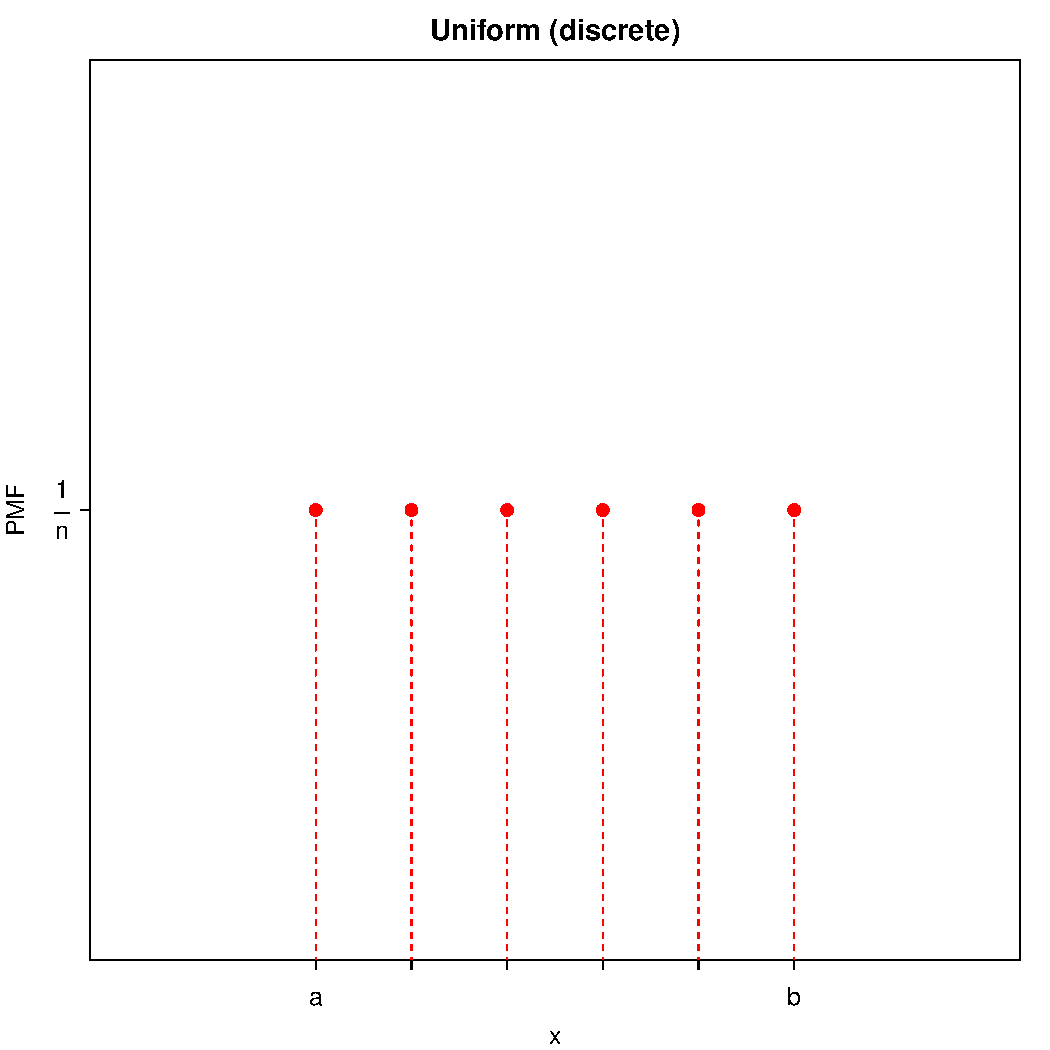
\includegraphics[scale=0.35]{figs/uniform-discrete.pdf}
  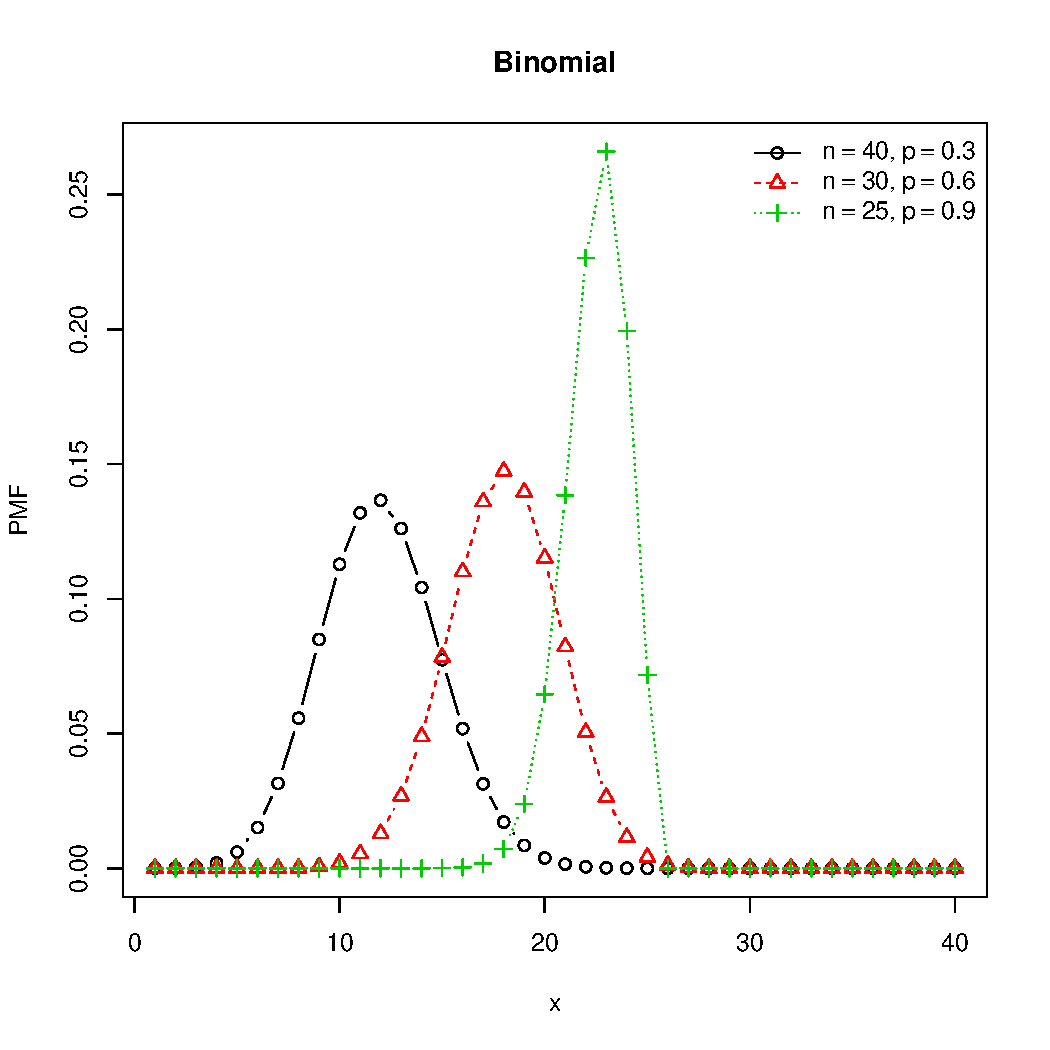
\includegraphics[scale=0.35]{figs/binomial.pdf}
  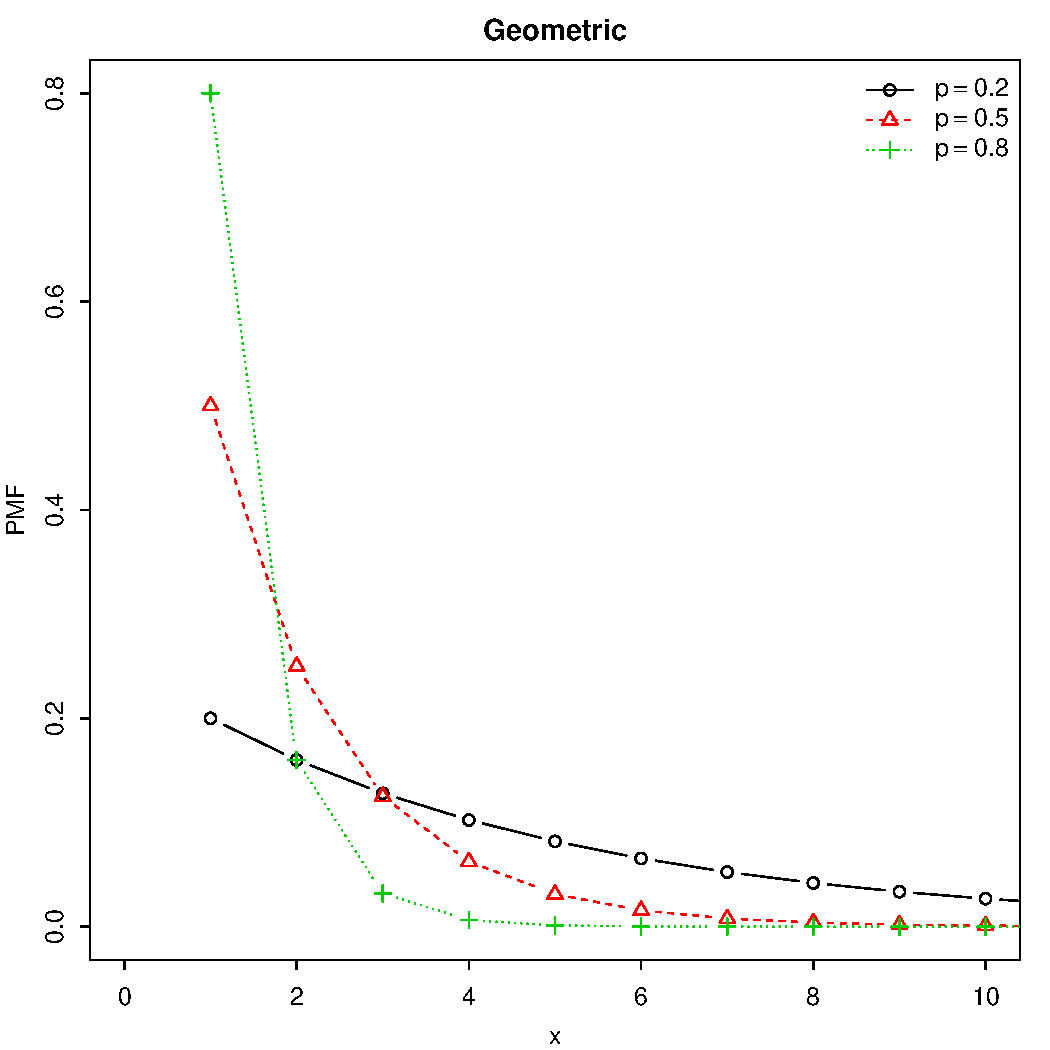
\includegraphics[scale=0.35]{figs/geometric.pdf}
  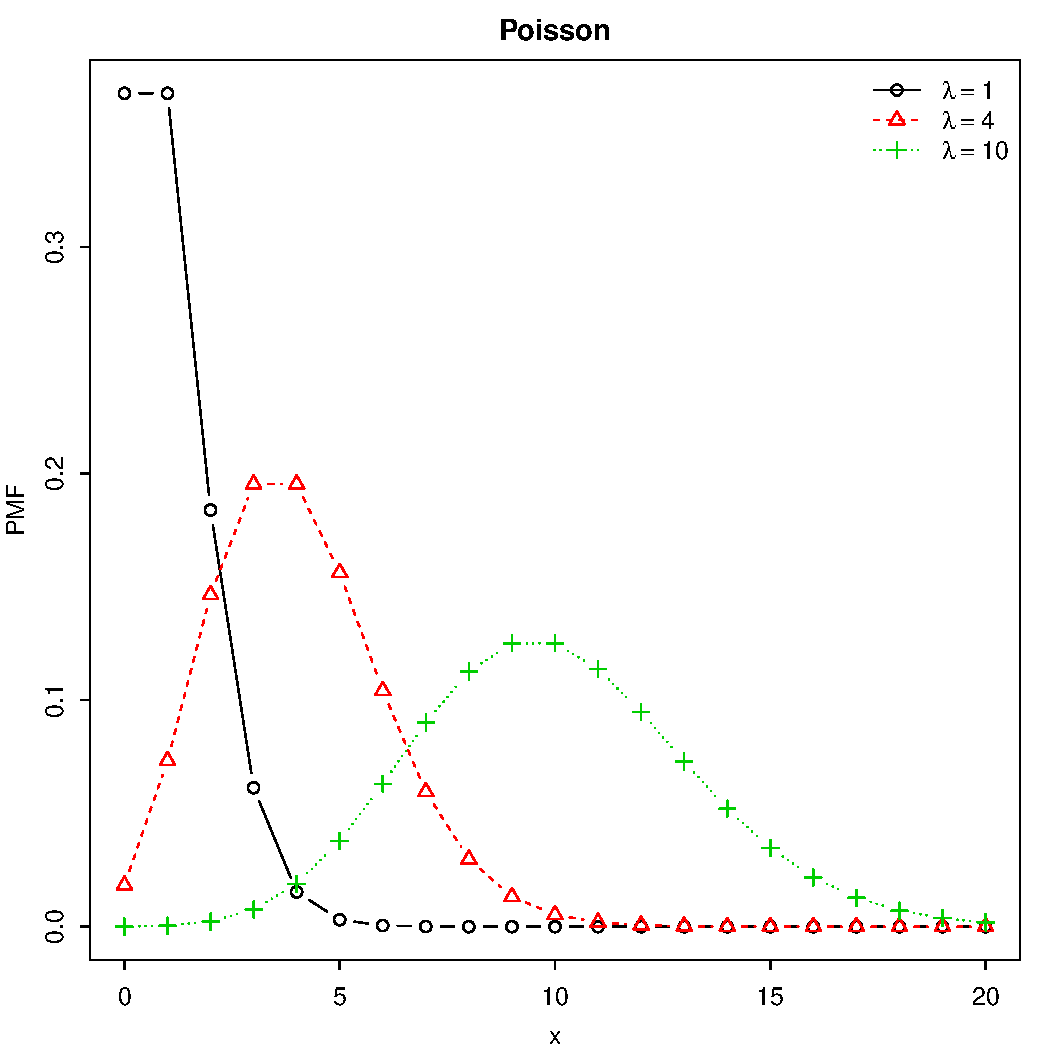
\includegraphics[scale=0.35]{figs/poisson.pdf}
\end{figure}

\end{center}

\footnotetext{\T{Footnote about notation}}

\pagebreak

\subsection{\T{Continuous Distributions}}

\begin{center}
\small
%\newcolumntype{L}{>{\varwidth[c]{\linewidth}}l<{\endvarwidth}}
\newcolumntype{M}{>{\begin{math}\displaystyle}c<{\end{math}}}
\begin{tabular}{@{}l*6{M}@{}}
  \toprule &&&&&& \\[-2ex]
  & \text{\T{Notation}}
  & F_X(x) & f_X(x) & \E{X} & \V{X} & M_X(s) \\[1ex]

  \midrule

  \T{Uniform} & \unif & \punif & \dunif &
  \frac{a+b}{2} & \frac{(b-a)^2}{12} &
  \frac{e^{sb}-e^{sa}}{s(b-a)} \\[3ex]

  \T{Normal} & \norm &
  \Phi(x)=\displaystyle\int_{-\infty}^x \phi(t)\,dt &
  \phi(x)=\dnorm &
  \mu & \sigma^2 &
  \Exp{\mu s + \frac{\sigma^2s^2}{2}}\\[3ex]

  \T{Log-Normal} & \ln\norm&
  \frac{1}{2}+\frac{1}{2} \erf\left[\frac{\ln x-\mu}{\sqrt{2\sigma^2}}\right] &
  \frac{1}{x\sqrt{2\pi\sigma^2}} \Exp{-\frac{(\ln x - \mu)^2}{2\sigma^2}} &
  e^{\mu+\sigma^2/2} &
  (e^{\sigma^2}-1) e^{2\mu+\sigma^2} &
  \\[3ex]

  \T{Multivariate Normal} & \mvn & &
  (2\pi)^{-k/2} |\Sigma|^{-1/2} e^{-\frac{1}{2}(x-\mu)^T \Sigma^{-1}(x-\mu)} &
  \mu & \Sigma &
  \Exp{\mu^T s + \frac{1}{2} s^T \Sigma s}\\[3ex]

  \T{Student's t} & \text{Student}(\nu)
  & I_x\left( \frac{\nu}{2},\frac{\nu}{2} \right)
  & \frac{\Gamma\left(\frac{\nu+1}{2}\right)}
    {\sqrt{\nu\pi}\Gamma\left(\frac{\nu}{2}\right)}
    \left(1+\frac{x^2}{\nu}\right)^{-(\nu+1)/2}
  & 0 %\; \nu > 1
  & \begin{cases}
      \displaystyle\frac{\nu}{\nu-2} & \nu > 2 \\
      \infty & 1 < \nu \le 2
    \end{cases}
  & \\[3ex]

  \T{Chi-square} & \chisq &
  \frac{1}{\Gamma(k/2)} \gamma\left(\frac{k}{2}, \frac{x}{2}\right) &
  \frac{1}{2^{k/2} \Gamma(k/2)} x^{k/2-1} e^{-x/2}&
  k & 2k &
  (1-2s)^{-k/2} \; s<1/2\\[3ex]

  F & \text{F}(d_1,d_2) &
  I_\frac{d_1x}{d_1x+d_2}\left(\frac{d_1}{2},\frac{d_1}{2}\right) &
  \frac{\sqrt{\frac{(d_1x)^{d_1} d_2^{d_2}}{(d_1x+d_2)^{d_1+d_2}}}}
    {x\mathrm{B}\left(\frac{d_1}{2},\frac{d_1}{2}\right)} &
  \frac{d_2}{d_2-2} %\; d_2 > 2
  & \frac{2d_2^2(d_1+d_2-2)}{d_1(d_2-2)^2(d_2-4)} %\; d_2 > 4
  & \\[3ex]

  \T{Exponential} & \ex & \pex & \dex &
  \beta & \beta^2 &
  \frac{1}{1-\beta s} \left(s < 1/\beta \right) \\[3ex]

  Gamma & \gam &
  \frac{\gamma(\alpha,x/\beta)}{\Gamma(\alpha)} & \dgamma &
  \alpha\beta & \alpha\beta^2 &
  \left( \frac{1}{1-\beta s} \right)^\alpha \left( s < 1/\beta \right)\\[3ex]

  \T{Inverse Gamma} & \invgamma & \pinvgamma & \dinvgamma &
  \frac{\beta}{\alpha-1} \; \alpha>1 &
  \frac{\beta^2}{(\alpha-1)^2(\alpha-2)^2} \; \alpha > 2 &
  \frac{2(-\beta s)^{\alpha/2}}{\Gamma(\alpha)}K_\alpha
  \left( \sqrt{-4\beta s} \right)\\[3ex]

  Dirichlet & \dir & & \ddir &
  \frac{\alpha_i}{\sum_{i=1}^k \alpha_i} &
  \frac{\E{X_i}(1-\E{X_i})}{\sum_{i=1}^k\alpha_i + 1} & \\[3ex]

  Beta & \bet & I_x(\alpha,\beta)& \dbeta &
  \frac{\alpha}{\alpha+\beta} &
  \frac{\alpha\beta}{(\alpha+\beta)^2(\alpha+\beta+1)} &
  1+\sum_{k=1}^{\infty} \left( \prod_{r=0}^{k-1}
    \frac{\alpha+r}{\alpha+\beta+r} \right) \frac{s^k}{k!} \\[3ex]

  Weibull & \mathrm{Weibull}(\lambda, k) & 1 - e^{-(x/\lambda)^k} & \dweibull &
  \lambda \Gamma\left(1 + \frac{1}{k} \right) &
  \lambda^2 \Gamma\left(1 + \frac{2}{k}\right) - \mu^2 &
  \sum_{n=0}^\infty \frac{s^n \lambda^n}{n!} \Gamma\left(1+\frac{n}{k}\right)
  \\[3ex]

  Pareto & \mathrm{Pareto}(x_m, \alpha) &
  1 - \left(\frac{x_m}{x} \right)^\alpha \; x\ge x_m &
  \alpha\frac{x_m^\alpha}{x^{\alpha+1}} \quad x\ge x_m&
  \frac{\alpha x_m}{\alpha-1} \; \alpha>1 &
  \frac{x_m^\alpha}{(\alpha-1)^2(\alpha-2)} \; \alpha>2 &
  \alpha(-x_m s)^\alpha \Gamma(-\alpha,-x_m s) \; s<0\\[3ex]

  \bottomrule
\end{tabular}
\end{center}

\begin{figure}[H]
  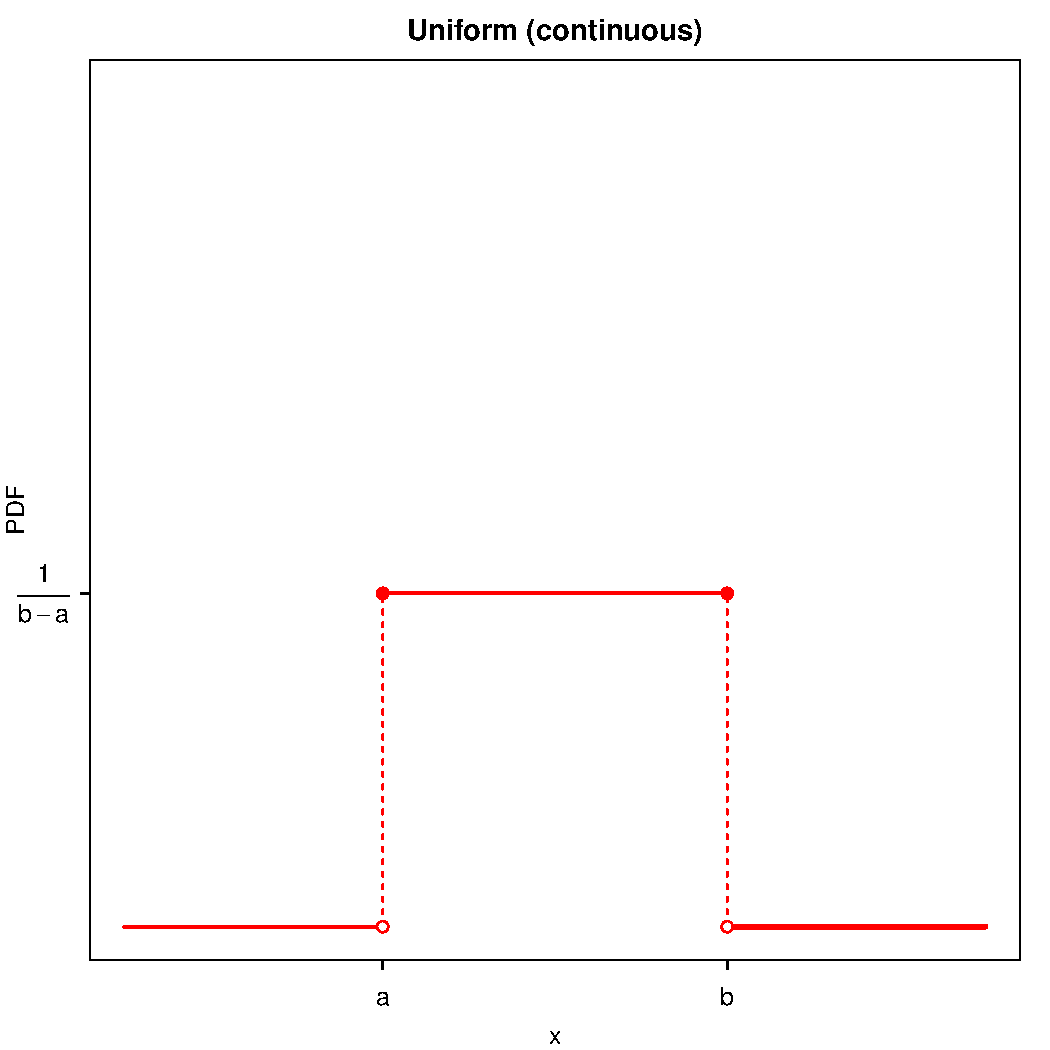
\includegraphics[scale=0.35]{figs/uniform-continuous.pdf}
  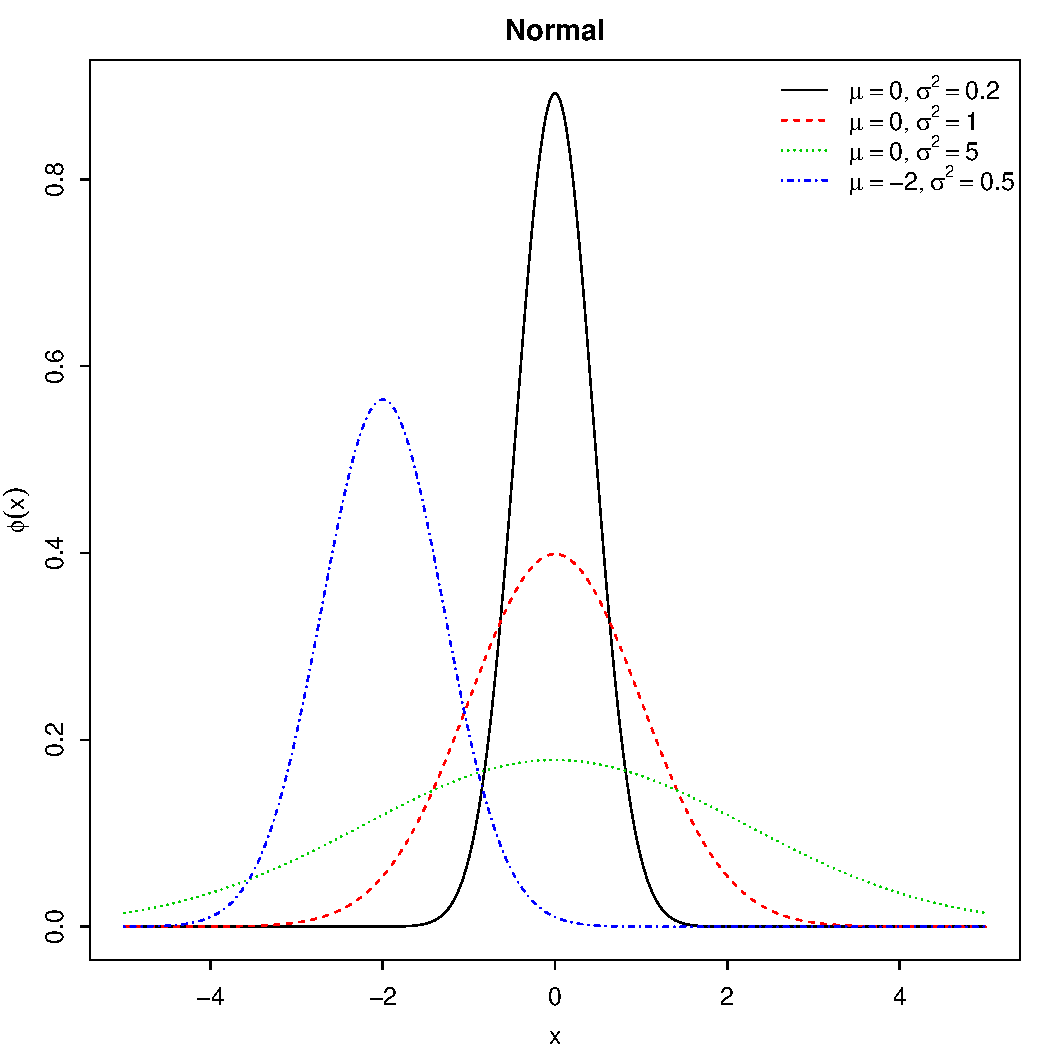
\includegraphics[scale=0.35]{figs/normal.pdf}
  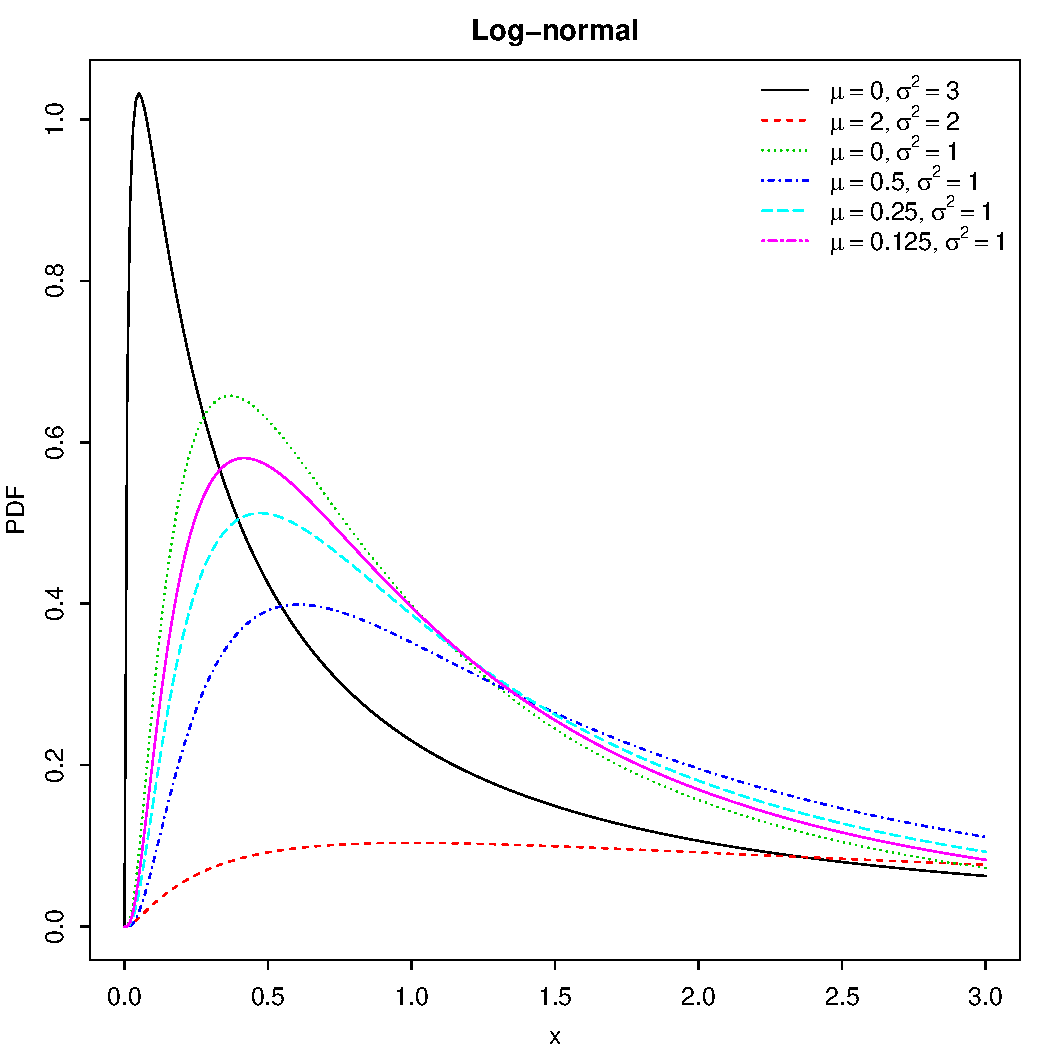
\includegraphics[scale=0.35]{figs/lognormal.pdf}
  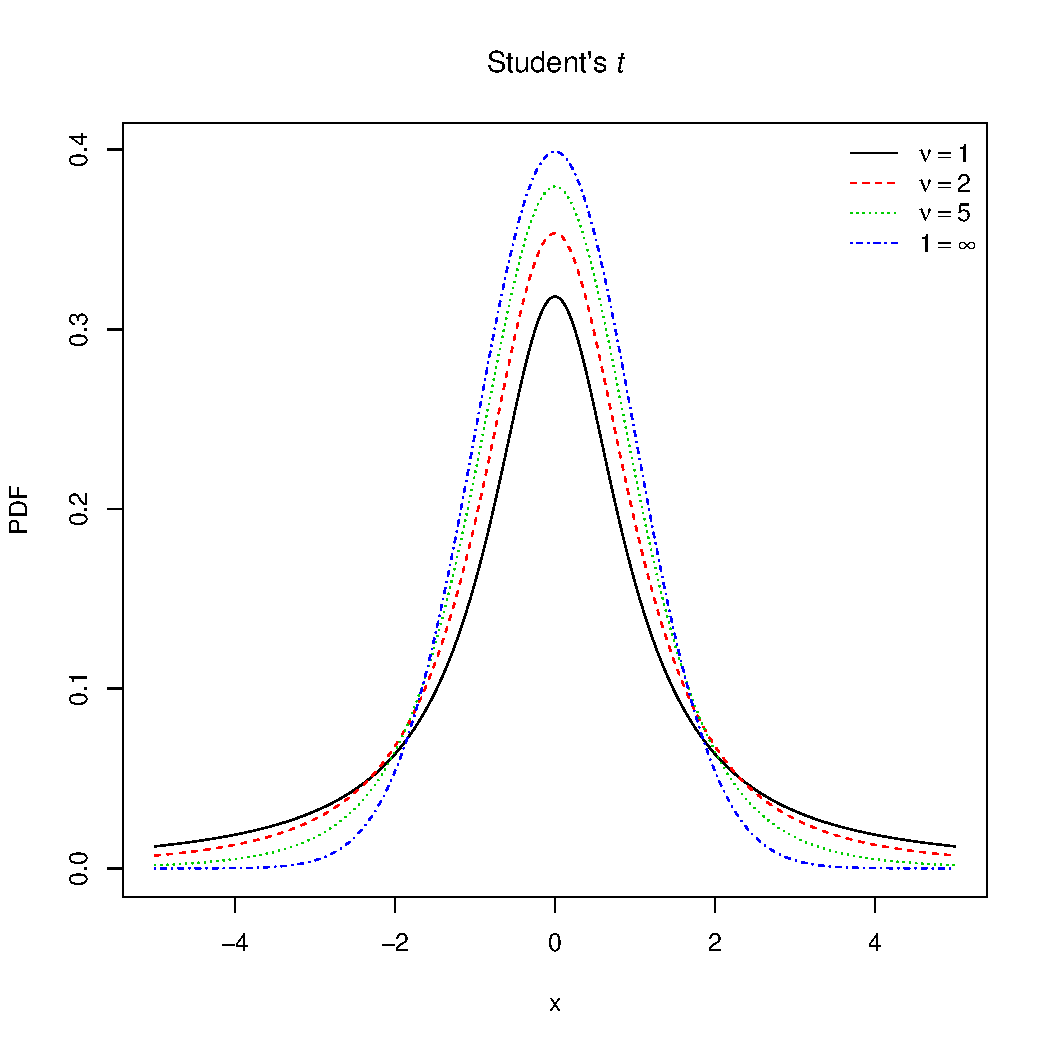
\includegraphics[scale=0.35]{figs/student.pdf}
  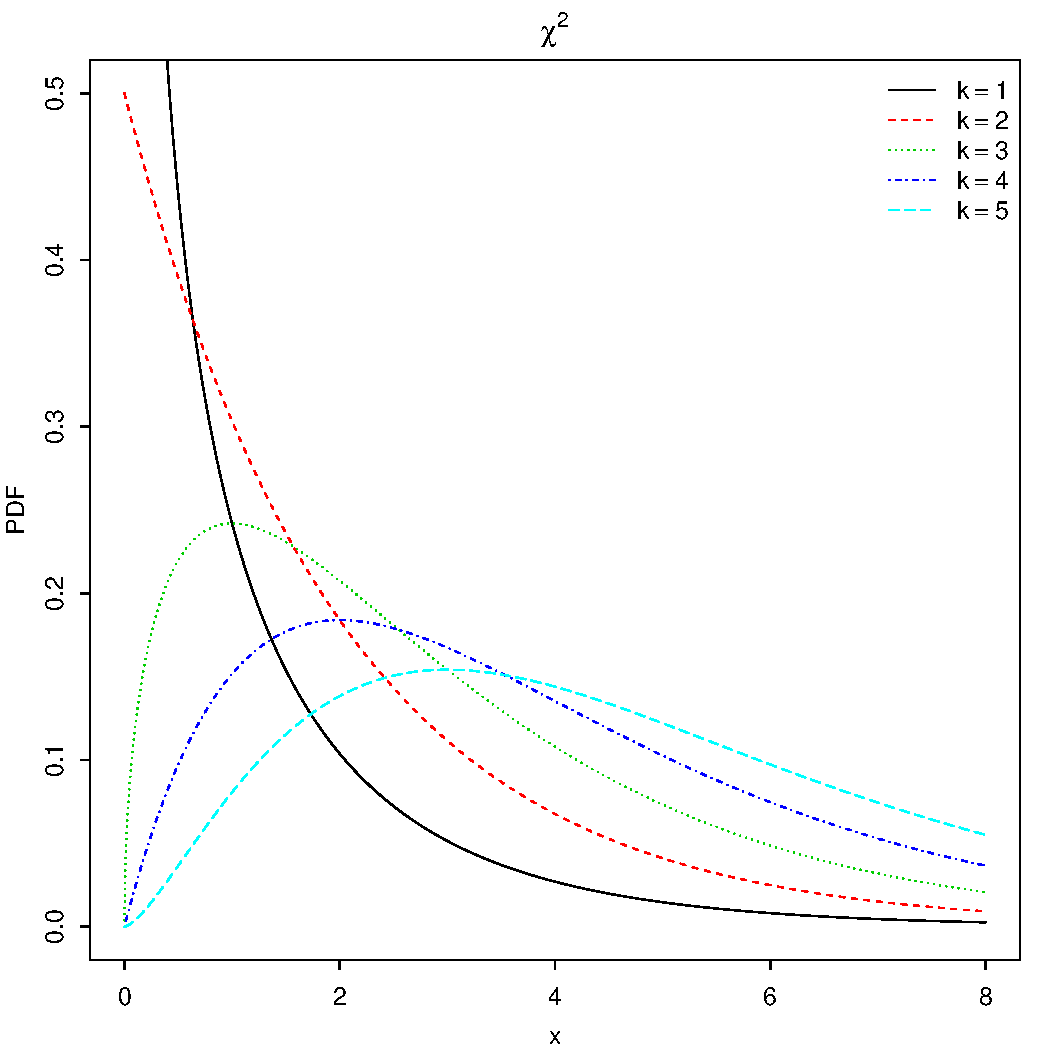
\includegraphics[scale=0.35]{figs/chisquare.pdf}
  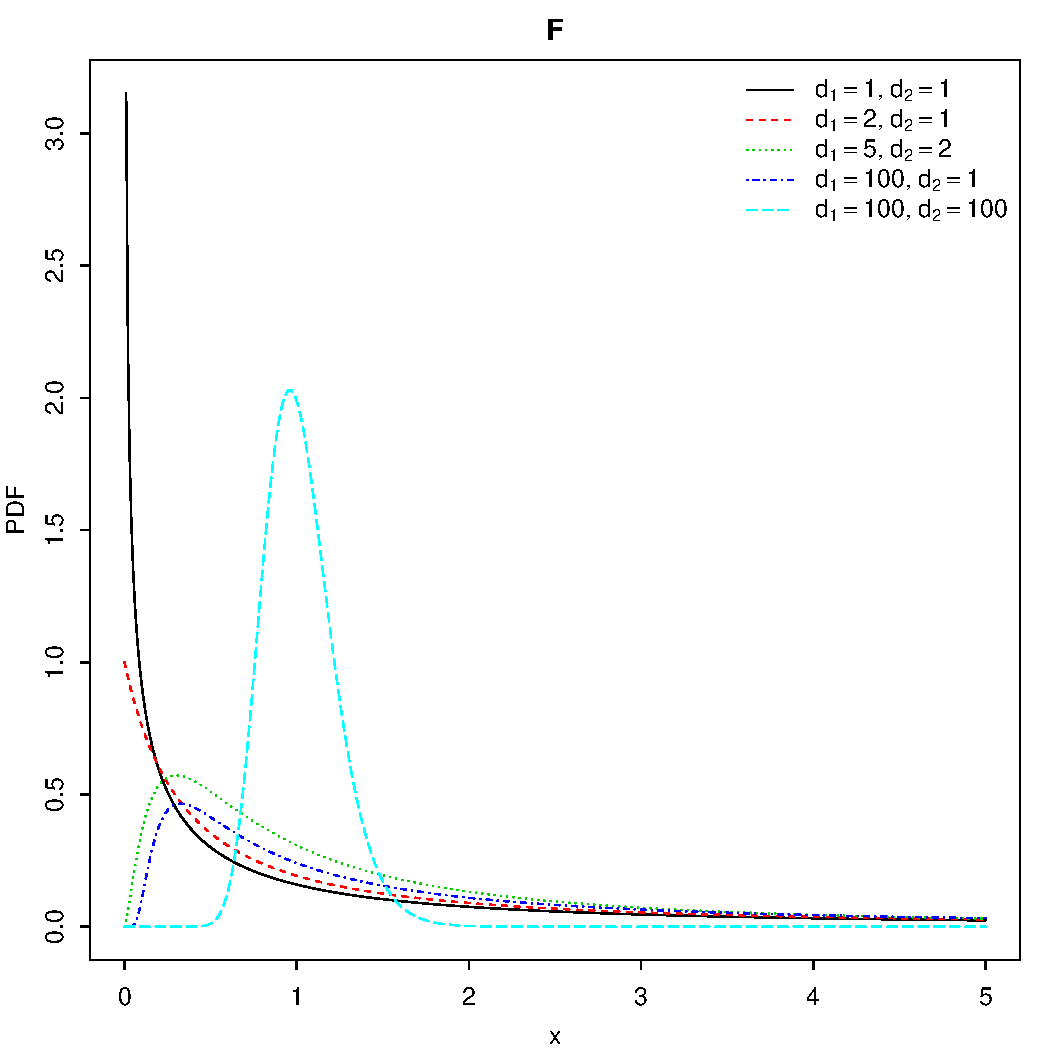
\includegraphics[scale=0.35]{figs/f.pdf}
  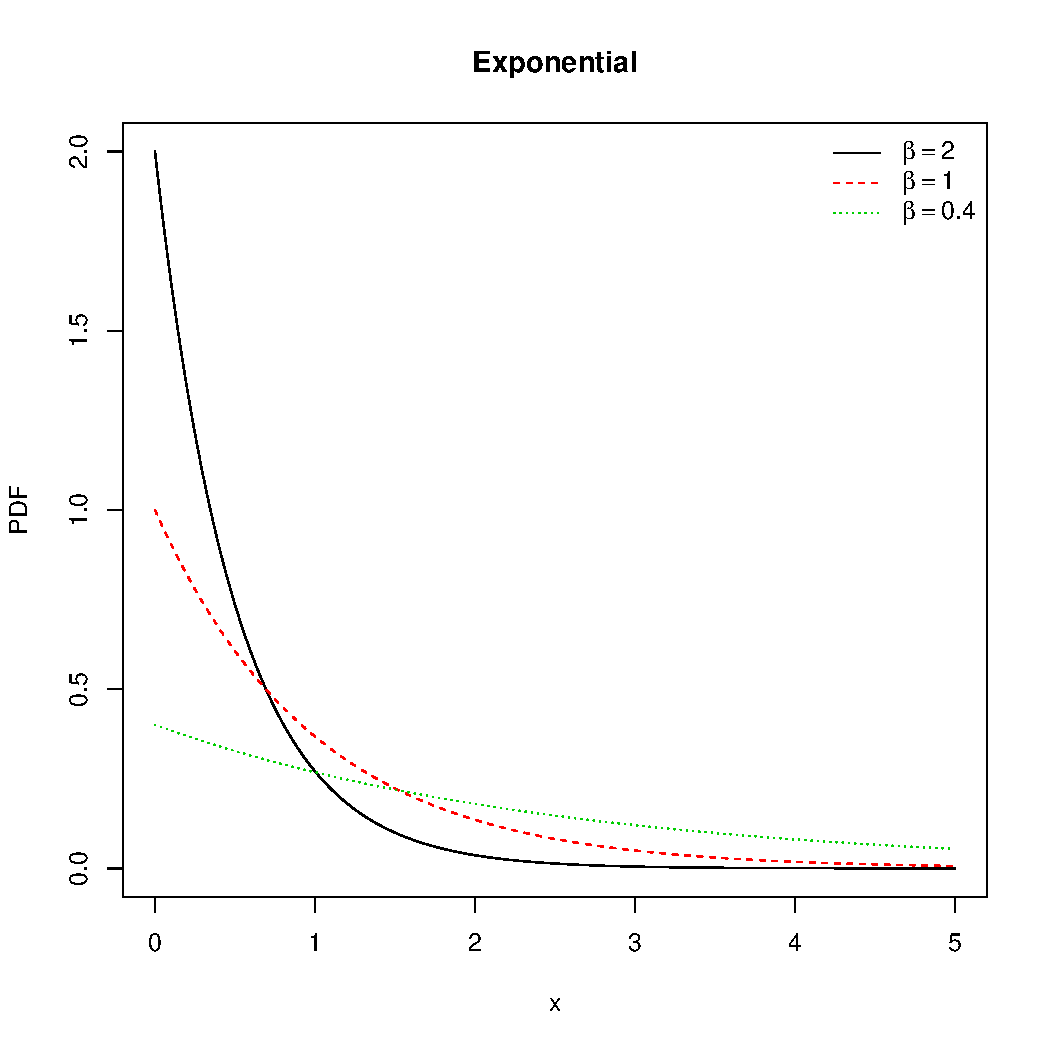
\includegraphics[scale=0.35]{figs/exponential.pdf}
  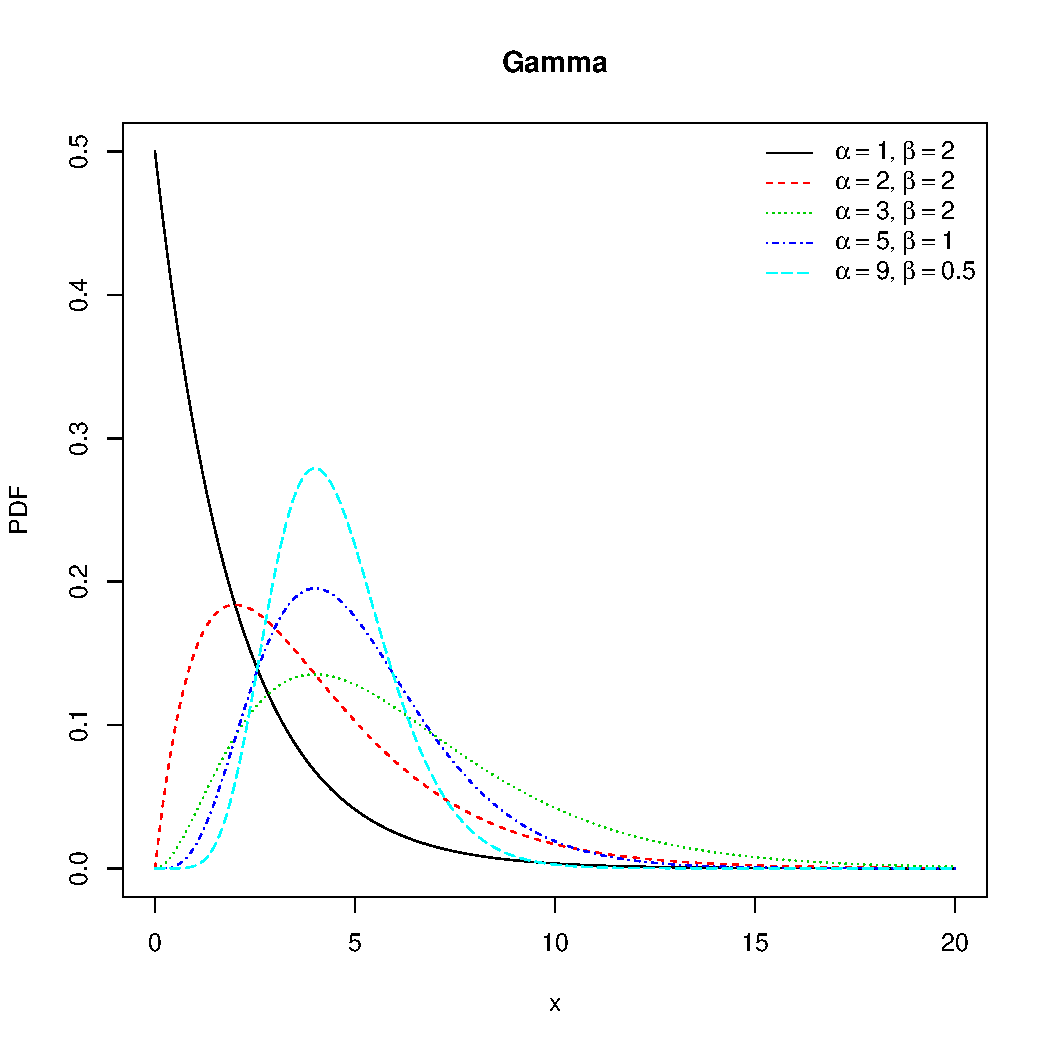
\includegraphics[scale=0.35]{figs/gamma.pdf}
  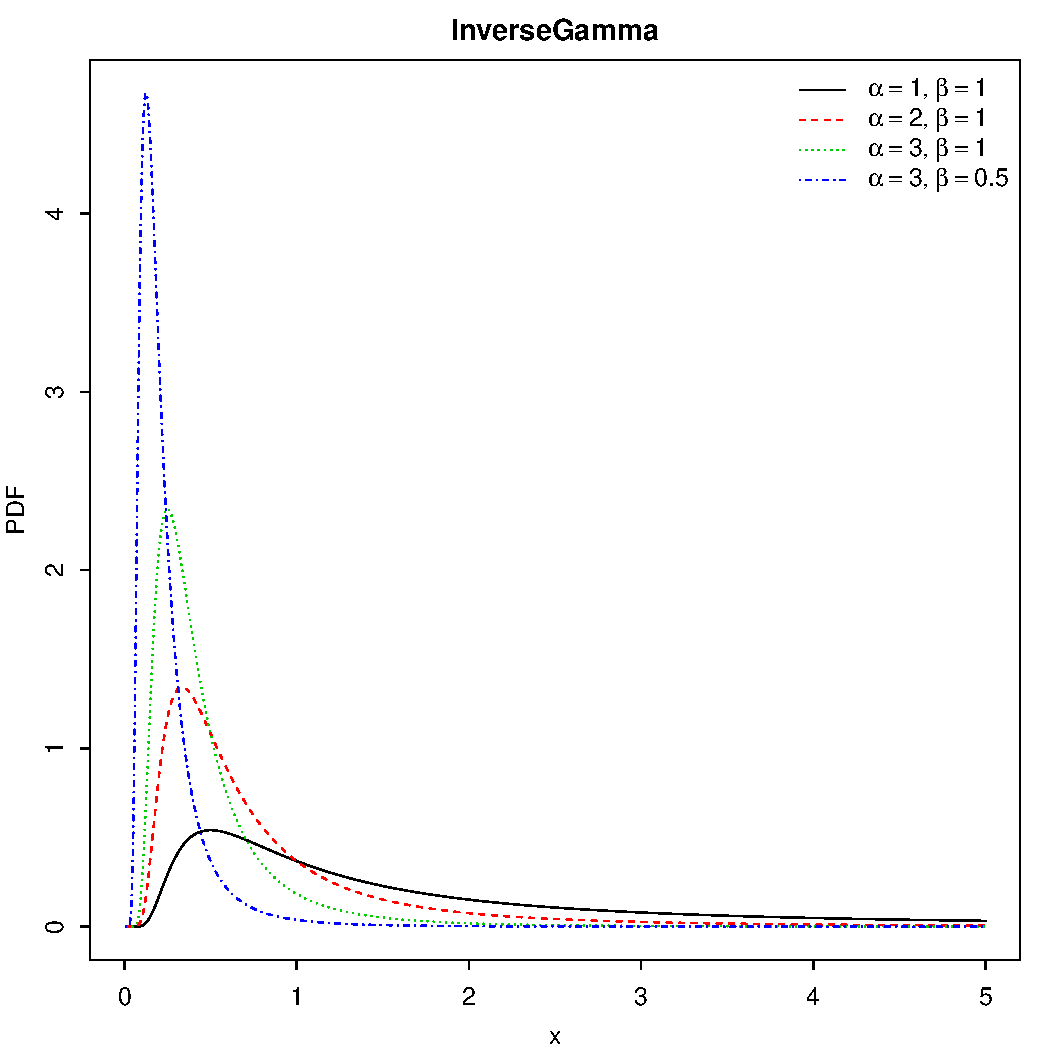
\includegraphics[scale=0.35]{figs/invgamma.pdf}
  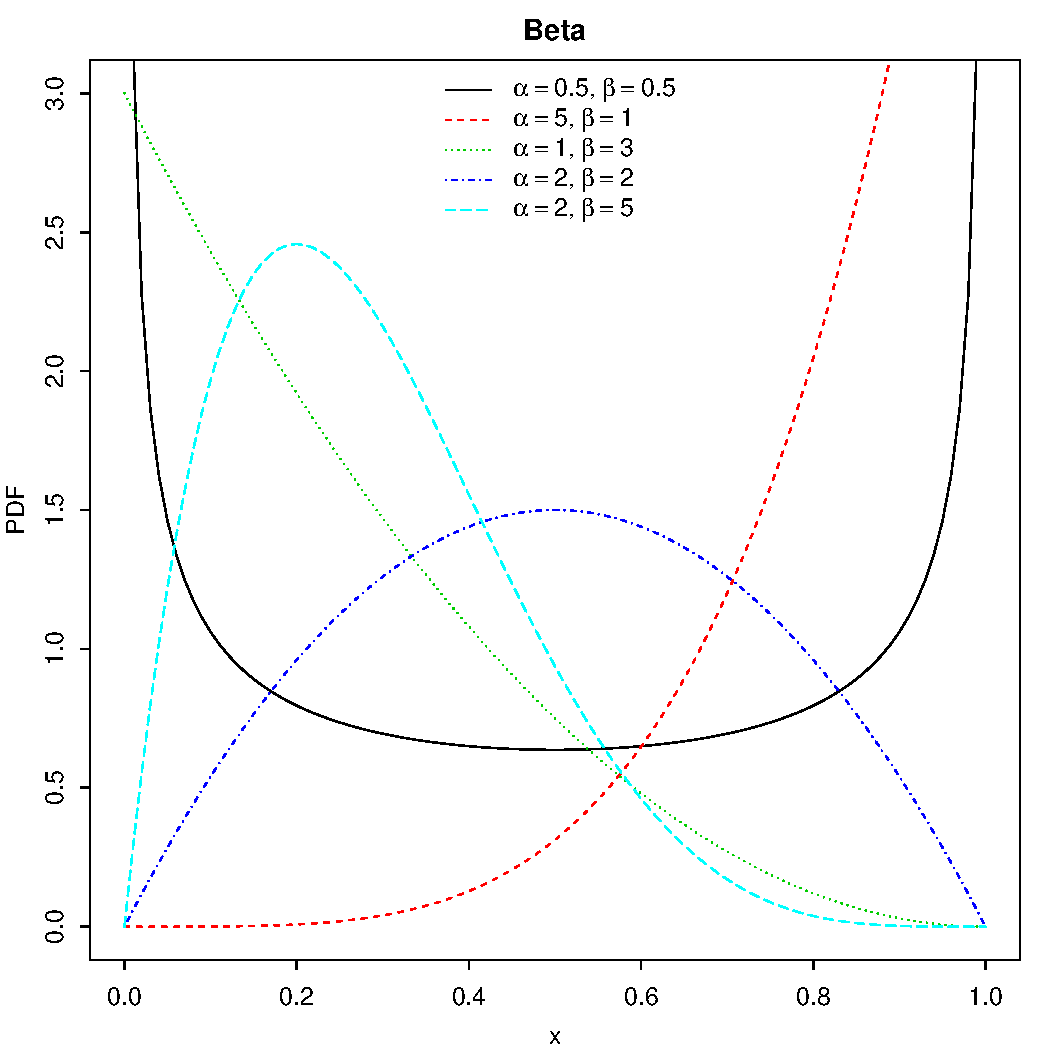
\includegraphics[scale=0.35]{figs/beta.pdf}
  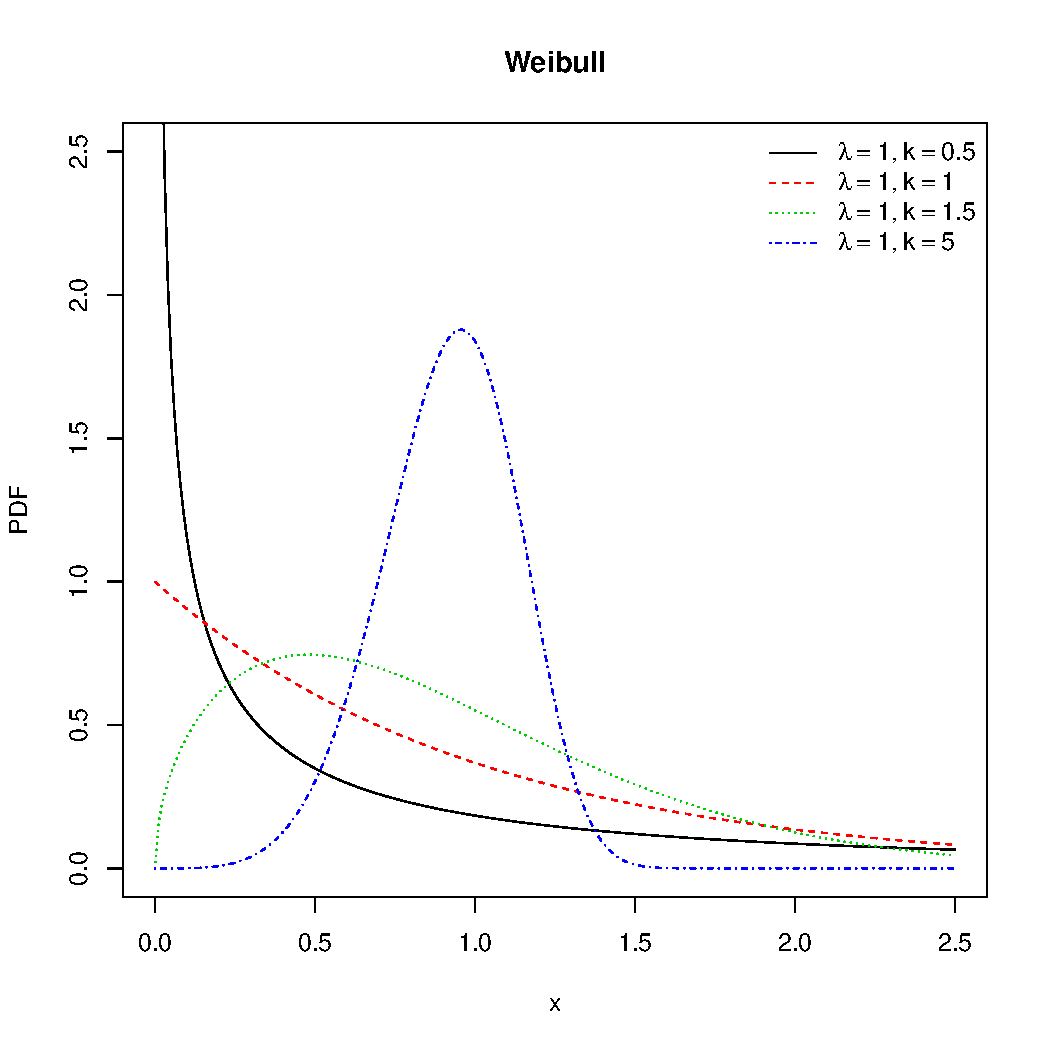
\includegraphics[scale=0.35]{figs/weibull.pdf}
  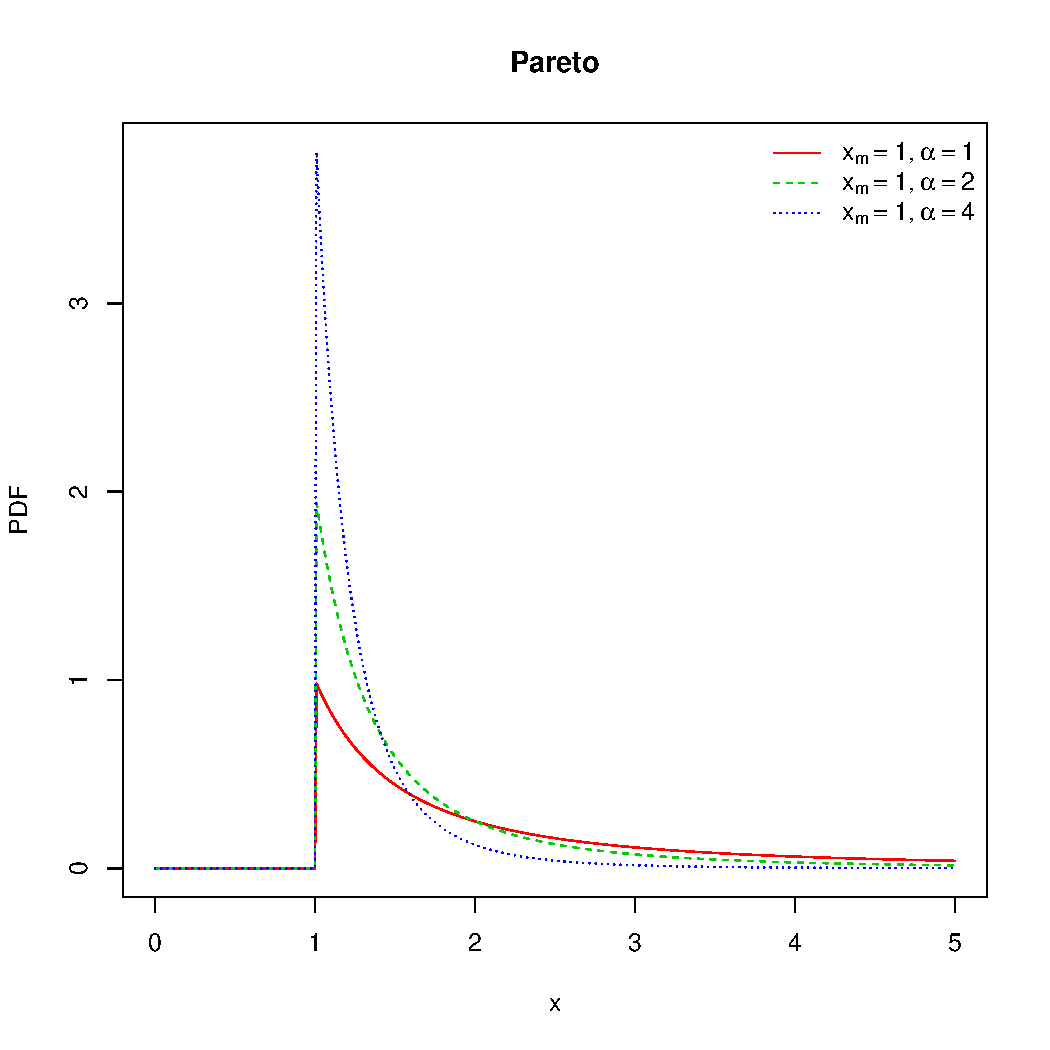
\includegraphics[scale=0.35]{figs/pareto.pdf}
\end{figure}

\begin{multicols*}{2}

\section{\T{Probability Theory}}

\T{Definitions}
\begin{itemize}
  \item \T{Sample space} $\Omega$
  \item \T{Outcome} $\omega \in \Omega$
  \item \T{Event} $A \subseteq \Omega$
  \item \T{Sigma-algebra} $\mathcal{A}$
    \begin{enumerate}
      \item $\emptyset \in \mathcal{A}$
      \item $A_1,A_2,\dots, \in \mathcal{A}
        \imp \bigcup_{i=1}^\infty A_i \in \mathcal{A}$
      \item $A \in \mathcal{A} \imp \comp{A} \in \mathcal{A}$
    \end{enumerate}
  \item \T{Probability Distribution} $\prob$
    \begin{enumerate}
      \item $\Pr{A} \ge 0 \quad \forall A$
      \item $\Pr{\Omega} = 1$
      \item $\Pr{\displaystyle\bigsqcup_{i=1}^\infty A_i}
        = \displaystyle\sum_{i=1}^\infty \Pr{A_i}$
    \end{enumerate}
  \item \T{Probability space} $(\Omega,\mathcal{A},\prob)$
\end{itemize}

\T{Properties}
\begin{itemize}
  \item $\Pr{\emptyset} = 0$
  \item $B = \Omega \cap B = (A \cup \comp{A}) \cap B
    = (A \cap B) \cup (\comp{A} \cap B)$
  \item $\Pr{\comp{A}} = 1 - \Pr{A}$
  \item $\Pr{B} = \Pr{A \cap B} + \Pr{\comp{A} \cap B}$
  \item $\Pr{\Omega} = 1 \qquad \Pr{\emptyset} = 0$
  \item $\comp{\left(\bigcup_n A_n\right)} = \bigcap_n \comp{A_n}
    \quad
    \comp{\left(\bigcap_n A_n\right)} = \bigcup_n \comp{A_n}
    \qquad$
    \textsc{DeMorgan}
  \item $\Pr{\bigcup_n A_n}
    = 1 - \Pr{\bigcap_n \comp{A_n}}$
  \item $\Pr{A \cup B} = \Pr{A} + \Pr{B} - \Pr{A \cap B}\\[1ex]
    \imp \Pr{A \cup B} \le \Pr{A} + \Pr{B}$
  \item $\Pr{A \cup B}
    = \Pr{A \cap \comp{B}} + \Pr{\comp{A} \cap B} + \Pr{A \cap B}$
  \item $\Pr{A \cap \comp{B}} = \Pr{A} - \Pr{A \cap B}$
\end{itemize}

\T{Continuity of Probabilities}
\begin{itemize}
  \item $A_1 \subset A_2 \subset \dots \imp \limn \Pr{A_n} = \Pr{A}
    \quad\text{\T{where}} A = \bigcup_{i=1}^\infty A_i$
  \item $A_1 \supset A_2 \supset \dots \imp \limn \Pr{A_n} = \Pr{A}
    \quad\text{\T{where}} A = \bigcap_{i=1}^\infty A_i$
\end{itemize}

\T{Independence} \ind
\[A \ind B \eqv \Pr{A \cap B} = \Pr{A}\Pr{B}\]

\T{Conditional Probability}
\[\Pr{A \giv B} = \frac{\Pr{A \cap B}}{\Pr{B}} \qquad \Pr{B} > 0\]

\T{Law of Total Probability}
\[ \Pr{B} = \sum_{i=1}^n \Pr{B|A_i}\Pr{A_i}
  \qquad \Omega = \bigsqcup_{i=1}^n A_i\]

\textsc{\T{Bayes' Theorem}}
\[\Pr{A_i \giv B}
= \frac{\Pr{B \giv A_i}\Pr{A_i}}{\sum_{j=1}^n \Pr{B \giv A_j}\Pr{A_j}}
\qquad \Omega = \bigsqcup_{i=1}^n A_i\]

\T{Inclusion-Exclusion Principle}
\[\biggl|\bigcup_{i=1}^n A_i\biggr| = \sum_{r=1}^n(-1)^{r-1}
  \sum_{i \le i_1 < \dots < i_r \le n}\biggl|\bigcap_{j=1}^r A_{i_j}\biggr|\]

\section{\T{Random Variables}}

\T{Random Variable}
\[X: \Omega \to \R\]

\T{Probability Mass Function}
\[f_X(x) = \Pr{X = x} = \Pr{\{\omega\in\Omega:X(\omega) = x\}}\]

\T{Probability Density Function}
\[\Pr{a \le X \le b} = \int_a^b f(x)\dx\]

\T{Cumulative Distribution Function}
\[F_X:\R \to [0,1] \qquad F_X(x) = \Pr{X \le x}\]

\begin{enumerate}
  \item \T{Nondecreasing}: $x_1 < x_2 \imp F(x_1) \le F(x_2)$
  \item \T{Normalized}: $\lim_{x\to -\infty} = 0$
    \T{and} $\lim_{x\to \infty} = 1$
  \item \T{Right-Continuous}: $\lim_{y\downarrow x} F(y) = F(x)$
\end{enumerate}

\[\Pr{a\le Y\le b \giv X=x} = \int_a^b f_{Y|X}(y\giv x) dy \qquad a \le b\]
\[ f_{Y|X}(y\giv x) = \frac{f(x,y)}{f_X(x)} \]

\T{Independence}
\begin{enumerate}
  \item $\Pr{X \le x, Y \le y} = \Pr{X \le x}\Pr{Y \le y}$
  \item $f_{X,Y}(x,y) = f_X(x)f_Y(y)$
\end{enumerate}

\subsection{\T{Transformations}}

\T{Transformation function}
\[Z = \transform(X)\]

\T{Discrete}
\[f_Z(z) = \Pr{\transform(X) = z} = \Pr{\{x:\transform(x) = z\}}
= \Pr{X \in \transform^{-1}(z)} = \sum_{x \in \transform^{-1}(z)} \!\!\!f(x)\]

\T{Continuous}
\[F_Z(z) = \Pr{\transform(X) \le z} = \int_{A_z} f(x) \dx \quad
    \text{with } A_z = \{x:\transform(x) \le z\}\]

\T{Special case if transform strictly monotone}
\[f_Z(z)
    = f_X(\transform^{-1}(z))
      \left|\frac{d}{dz}\transform^{-1}(z)\right|
    = f_X(x)\left|\frac{dx}{dz}\right|
    = f_X(x)\frac{1}{|J|}\]

\T{The Rule of the Lazy Statistician}
\[\E{Z} = \int \transform(x) \dfx\]
\[\E{I_A(x)} = \int I_A(x) \dfx = \int_A \dfx = \Pr{X \in A}\]

\T{Convolution}
\begin{itemize}
  \item $ Z:=X+Y \qquad
    f_Z(z)=\displaystyle\int_{-\infty}^{\infty} f_{X,Y}(x,z-x)\,dx
    \;\stackrel{X,Y \ge 0}{=}\; \int_0^z f_{X,Y}(x,z-x)\,dx$
  \item $ Z:=|X-Y| \qquad
    f_Z(z)=\displaystyle2\int_0^\infty f_{X,Y}(x,z+x)\,dx$
    %\;\stackrel{X,Y \ge 0}{=}\; \int_0^\infty f_{X,Y}(x,z+x)\,dx$
  \item $ Z:=\displaystyle\frac{X}{Y} \qquad
    f_Z(z)=\displaystyle\int_{-\infty}^{\infty} |x| f_{X,Y}(x,xz)\,dx
    \;\stackrel{\ind}{=}\; \int_{-\infty}^{\infty} xf_x(x)f_X(x)f_Y(xz)\,dx$
\end{itemize}

%  \subsection{Joint Distribution}
%  \begin{itemize}
%    \item $f(x,y) = \Pr{X \le k, Y \le m)}
%      = \displaystyle\int_{-\infty}^k\int_{-\infty}^m f(x,y)\,dy\,dx$
%    \item $\Pr{a < X \le b, c < y \le d} = F(b,d) - F(a,d) - F(b,c) + F(a,c)$
%    \item $f_X(x) = \displaystyle\int_{-\infty}^\infty f(x,y)\,dy \qquad
%      f_Y(y) = \displaystyle\int_{-\infty}^\infty f(x,y)\,dx$
%  \end{itemize}

%  Order Statistics
%  \begin{itemize}
%    \item $U_i\ind U_j$ continuous \textsc{RVs} with common density $f$
%    \item $X_1(\omega) < \dots < X_n(\omega)$ permuted set of $U_i$'s
%    \item $X_k = $ \emph{k$^{th}$ order statistic}
%    \item $X_1(\omega) = \min(U_1(\omega),\dots,U_n(\omega))$
%    \item $X_n(\omega) = \max(U_1(\omega),\dots,U_n(\omega))$
%    \item $R(\omega) = X_n(\omega) - X_1(\omega)$
%  \end{itemize}

\section{\T{Expectation}}

\T{Definition} \T{and} \T{properties}
\begin{itemize}
  \item $\E{X} = \mu_X = \displaystyle \int x \dfx =
    \begin{cases}
      \displaystyle\sum_x xf_X(x) & \text{X \T{discrete}} \\\\
      \displaystyle\int xf_X(x)\dx & \text{X \T{continuous}}
    \end{cases}$
  \item $\Pr{X=c}=1 \imp \E{X} = c$
  \item $\E{cX} = c\,\E{X}$
  \item $\E{X+Y} = \E{X}+\E{Y}$
  \item $\E{XY} = \displaystyle\int_{X,Y} xy f_{X,Y}(x,y)\dfx\dfy$
  \item $\E{\transform(Y)} \neq \transform(\E{X}) \qquad$
    (cf.~\hyperref[jensen]{\textsc{Jensen} \T{inequality}})
  \item $\Pr{X\ge Y} = 0 \imp \E{X}\ge\E{Y}
    \wedge \Pr{X=Y}=1 \imp \E{X}=\E{Y}$
%  \item $\Pr{\lvert Y\rvert\le c} = 1 \imp \E{Y}<\infty
%    \wedge \lvert\E{X}\rvert\le c$
  \item $\E{X} = \displaystyle\sum_{x=1}^\infty \Pr{X\ge x}$
\end{itemize}

\T{Sample mean}
\[\samplemean = \frac{1}{n}\sum_{i=1}^n X_i\]

\begin{titemize}{\T{Conditional expectation}}
  \item $\E{Y\giv X=x} = \displaystyle\int y f(y\giv x)\dy$
  \item $\E{X} = \E{\E{X\giv Y}}$
  \item $E[\transform(X,Y)\giv X=x]
    = \displaystyle\int_{-\infty}^\infty \transform(x,y)f_{Y|X}(y\giv x)\dx$
  \item $\E{\transform(Y,Z)\giv X=x} =
    \displaystyle\int_{-\infty}^\infty\transform(y,z)
    f_{(Y,Z)|X}(y,z\giv x)\,dy\,dz$
  \item $\E{Y+Z\giv X} = \E{Y\giv X} + \E{Z\giv X}$
  \item $\E{\transform(X)Y\giv X} = \transform(X)\E{Y\giv X}$
  \item $E[Y\giv X] = c \imp \cov{X,Y}=0$
\end{titemize}

\section{\T{Variance}}

\begin{titemize}{\T{Definition} \T{and} \T{properties}}
  \item $\V{X} = \sigma_X^2 = \E{(X-\E{X})^2} = \E{X^2} - \E{X}^2$
  \item $\V{\displaystyle\sum_{i=1}^n X_i} =
    \displaystyle\sum_{i=1}^n \V{X_i} + 2\sum_{i\ne j}\cov{X_i,Y_j}$
%    \stackrel{X_i \ind X_j}{=}\sum_{i=1}^n\V{X_i}$
  \item $\V{\displaystyle\sum_{i=1}^n X_i} =
    \displaystyle\sum_{i=1}^n\V{X_i} \quad$ if $X_i \ind X_j$
\end{titemize}

\T{Standard deviation}
\[\sd[X] = \sqrt{\V{X}} = \sigma_X\]

\T{Covariance}
\begin{itemize}
  \item $\cov{X,Y} = \E{(X-\E{X})(Y-\E{Y})} = \E{XY}-\E{X}\E{Y}$
  \item $\cov{X,a} = 0$
  \item $\cov{X,X} = \V{X}$
  \item $\cov{X,Y} = \cov{Y,X}$
  \item $\cov{aX,bY} = ab\cov{X,Y}$
  \item $\cov{X+a,Y+b} = \cov{X,Y}$
  \item $\cov{\displaystyle\sumin X_i, \sumjm Y_j}
    = \displaystyle\sumin\sumjm\cov{X_i, Y_j}$
\end{itemize}

\T{Correlation}
\[\corr{X,Y} = \displaystyle\frac{\cov{X,Y}}{\sqrt{\V{X}\V{Y}}}\]

\T{Independence}
\[X\ind Y \imp \corr{X,Y} = 0 \eqv \cov{X,Y} = 0 \eqv \E{XY}=\E{X}\E{Y}\]

\T{Sample variance}
\[\samplevar = \frac{1}{n-1}\sum_{i=1}^n(X_i-\samplemean)^2\]

\T{Conditional variance}
\begin{itemize}
  \item $\V{Y\giv X} = \E{(Y-\E{Y\giv X})^2\giv X} =\E{Y^2\giv X}-\E{Y\giv X}^2$
  \item $\V{Y} = \E{\V{Y\giv X}}+\V{\E{Y\giv X}}$
\end{itemize}

\section{\T{Inequalities}}

\textsc{Cauchy-Schwarz}
\[\E{XY}^2 \le \E{X^2}\E{Y^2}\]

\textsc{Markov}
\[\Pr{\transform(X) \ge t}\le\frac{\E{\transform(X)}}{t}\]

\textsc{Chebyshev}
\[\Pr{\lvert X-\E{X}\rvert \ge t} \le \frac{\V{X}}{t^2}\]

\textsc{Chernoff}
\[\Pr{X \ge (1+\delta)\mu}
\le \left(\frac{e^\delta}{(1+\delta)^{1+\delta}}\right) \quad \delta>-1\]

\textsc{Jensen}\label{jensen}
\[\E{\transform(X)} \ge \transform(\E{X}) \quad
  \transform \text{ \T{convex}}\]

\section{\T{Distribution Relationships}}

\T{Binomial}
\begin{itemize}
  \item $X_i \dist \bern \imp \displaystyle\sum_{i=1}^n X_i \dist \bin$
  \item $X\dist\bin, Y\dist\bin[m,p] \imp X+Y\dist\bin[n+m,p]$
  \item $\limn\bin = \pois[np] \qquad$ ($n$ \T{large}, $p$ \T{small})
  \item $\limn\bin = \norm[np,np(1-p)] \qquad$
    ($n$ \T{large}, $p$ \T{far from 0 and 1})
\end{itemize}

\T{Negative Binomial}
\begin{itemize}
  \item $ X\dist \nbin[1,p] = \geo $
  \item $ X\dist \nbin[r,p] = \sum_{i=1}^r \geo $
  \item $X_i\dist \nbin[r_i,p] \imp \sum X_i\dist \nbin[\sum r_i,p] $
  \item $X\dist \nbin[r,p].\; Y\dist \bin[s+r,p] \imp \Pr{X\le s} = \Pr{Y\ge r}$
\end{itemize}

\T{Poisson}
\begin{itemize}
  \item $X_i\dist\pois[\lambda_i] \wedge X_i \ind X_j
    \imp \displaystyle\sumin X_i \dist \pois[\displaystyle\sumin \lambda_i]$
  \item $X_i\dist\pois[\lambda_i] \wedge X_i \ind X_j
    \imp X_i\,\left|\displaystyle\sumjn X_j\right. \dist
   \bin[\displaystyle\sumjn X_j,\displaystyle\frac{\lambda_i}{\sumjn\lambda_j}]$
\end{itemize}

Exponential
\begin{itemize}
%    \item $\forall n \in \mathbb N^+: X_i\dist\ex{\lambda}
  \item $X_i\dist\ex \wedge  X_i \ind X_j
    \imp \displaystyle\sumin X_i\dist \gam[n,\beta]$
  \item \T{Memoryless property}: $\Pr{X>x+y\giv X>y}=\Pr{X>x}$
\end{itemize}

\T{Normal}
\begin{itemize}
  \item $X\dist \norm[\mu,\sigma^2]
    \imp \left(\frac{X-\mu}{\sigma}\right)\dist\norm[0,1] $
  \item $X\dist \norm[\mu,\sigma^2] \wedge Z = aX+b
    \imp Z\dist\norm[a\mu+b,a^2\sigma^2] $
  \item $X\dist \norm[\mu_1,\sigma_1^2] \wedge Y\dist\norm[\mu_2,\sigma_2^2]
    \imp X+Y\,\dist \norm[\mu_1+\mu_2,\sigma_1^2 + \sigma_2^2] $
  \item $X_i\dist\norm[\mu_i,\sigma_i^2]
     \imp \sum_i X_i \dist \norm[\sum_i\mu_i,\sum_i\sigma_i^2]$
   \item $\Pr{a < X \le b}= \Phi\left(\frac{b-\mu}{\sigma}\right)
     - \Phi\left(\frac{a-\mu}{\sigma}\right) $
  \item $\Phi(-x) = 1 - \Phi(x) \qquad \phi'(x) = -x\phi(x) \qquad
    \phi''(x) = (x^2-1)\phi(x)$
  \item \T{Upper quantile of} $\norm[0,1]$: $z_{\alpha} = \Phi^{-1}(1-\alpha)$
\end{itemize}

Gamma
\begin{itemize}
  \item $X\dist\gam \eqv X/\beta \dist\gam[\alpha,1]$
  \item $\gam\dist \sum_{i=1}^\alpha\ex$
  \item $X_i\dist\gam[\alpha_i,\beta] \wedge X_i \ind X_j \imp
    \sum_i X_i\dist \gam[\sum_i \alpha_i,\beta]$
  \item $\displaystyle\frac{\Gamma(\alpha)}{\lambda^\alpha}
    = \displaystyle\int_0^\infty x^{\alpha-1} e^{-\lambda x} \dx$
\end{itemize}

Beta
\begin{itemize}
  \item $\displaystyle
    \frac{1}{\text{B}(\alpha,\beta)}x^{\alpha-1}(1-x)^{\beta-1}
    = \frac{\Gamma(\alpha+\beta)}{\Gamma(\alpha)\Gamma(\beta)}
    x^{\alpha-1}(1-x)^{\beta-1} $
  \item $\E{X^k}
    = \displaystyle\frac{\text{B}(\alpha+k,\beta)}{\text{B}(\alpha,\beta)}
    = \displaystyle\frac{\alpha+k-1}{\alpha+\beta+k-1}\E{X^{k-1}}$
  \item $\bet[1,1] \dist \unif[0,1]$
\end{itemize}

\section{\T{Probability and Moment Generating Functions}}

\begin{itemize}
  \item $G_X(t) = \E{t^X} \qquad |t| < 1$
  \item $M_X(t) = G_X(e^t) = \E{e^{Xt}}
    = \E{ \displaystyle\sum_{i=0}^\infty \frac{(Xt)^i}{i!}}
    = \displaystyle\sum_{i=0}^\infty \frac{\E{X^i}}{i!}\cdot t^i$
  \item $\Pr{X=0} = G_X(0)$
  \item $\Pr{X=1}=G_X'(0)$
  \item $\Pr{X=i} = \displaystyle\frac{G_X^{(i)}(0)}{i!}$
  \item $\E{X} = G_X'(1^-)$
  \item $\E{X^k} = M_X^{(k)}(0)$
  \item $\E{\displaystyle\frac{X!}{(X-k)!}} = G_X^{(k)}(1^-)$
  \item $\V{X} = G_X''(1^-) + G_X'(1^-)
    - \left(G_X'(1^-)\right)^2$
  \item $G_X(t) = G_Y(t) \imp X \stackrel{d}{=} Y$
\end{itemize}

\section{\T{Multivariate Distributions}}

\subsection{\T{Standard Bivariate Normal}}

\T{Let} $X,Y\dist\norm[0,1] \wedge X\ind Z$ \T{where}
$Y = \rho X + \sqrt{1-\rho^2}Z$\\

\T{Joint density}
\[
f(x,y) = \frac{1}{2 \pi \sqrt{1-\rho^2}}
\Exp{-\frac{x^2 + y^2 - 2\rho x y}{2 (1-\rho^2)}}
\]

\T{Conditionals}
\[
(Y\giv X=x) \dist \norm[\rho x,1-\rho^2] \qquad\text{and}\qquad
(X\giv Y=y) \dist \norm[\rho y,1-\rho^2]
\]

\T{Independence}
\[X \ind Y \eqv \rho = 0\]

\subsection{\T{Bivariate Normal}}
% - http://www.athenasc.com/Bivariate-Normal.pdf
% - http://mathworld.wolfram.com/BivariateNormalDistribution.html

\T{Let} $X\dist\norm[\mu_x,\sigma_x^2]$
  \T{and} $Y\dist\norm[\mu_y,\sigma_y^2]$.
\[f(x,y) = \frac{1}{2 \pi \sigma_x \sigma_y \sqrt{1-\rho^2}}
\Exp{-\frac{z}{2 (1-\rho^2)}}\]
\[ z =
  \left[
  \left(\frac{x-\mu_x}{\sigma_x}\right)^2
    + \left(\frac{y-\mu_y}{\sigma_y}\right)^2
    - 2\rho\left(\frac{x-\mu_x}{\sigma_x}\right)
      \left(\frac{y-\mu_y}{\sigma_y}\right)
  \right]
\]

\T{Conditional mean and variance}
\[\E{X\giv Y} = \E{X} + \rho\frac{\sigma_X}{\sigma_Y}(Y-\E{Y})\]
\[\V{X\giv Y} = \sigma_X \sqrt{1-\rho^2}\]

\subsection{\T{Multivariate Normal}}

\T{Covariance matrix} $\Sigma$ \quad (\T{Precision matrix} $\Sigma^{-1}$)
\[\Sigma =
  \begin{pmatrix}
  \V{X_1} & \cdots & \cov{X_1,X_k} \\
  \vdots & \ddots & \vdots \\
  \cov{X_k,X_1} & \cdots & \V{X_k}
  \end{pmatrix}\]

\T{If} $X \dist \norm[\mu,\Sigma]$,
\[f_X(x) = (2\pi)^{-n/2} \left|\Sigma\right|^{-1/2}
\Exp{-\frac{1}{2}(x-\mu)^T\Sigma^{-1}(x-\mu)} \]

\T{Properties}
\begin{itemize}
  \item $Z \dist \norm[0,1] \wedge X = \mu+\Sigma^{1/2}Z
    \imp X \dist \norm[\mu,\Sigma]$
  \item $X \dist \norm[\mu,\Sigma] \imp \Sigma^{-1/2}(X-\mu) \dist \norm[0,1]$
  \item $X \dist \norm[\mu,\Sigma] \imp AX \dist \norm[A\mu, A\Sigma A^T]$
  \item $X \dist \norm[\mu,\Sigma] \wedge \|a\| = k
    \imp a^TX \dist \norm[a^T\mu, a^T\Sigma a]$
\end{itemize}

\section{\T{Convergence}}

\T{Convergence Introduction}\\

\T{Types of Convergence}
\begin{enumerate}
  \item \T{In distribution}: $X_n \dconv X$
    \[\limn F_n(t) = F(t) \qquad
      \forall t \text{ \T{where} } F \text{ \T{continuous}}\]
  \item \T{In probability}: $X_n \pconv X$
    \[(\forall \varepsilon > 0) \;
    \lim_{n\to\infty} \Pr{|X_n -X| > \varepsilon} = 0\]
  \item \T{Almost surely}: $X_n \asconv X$
    \[\Pr{\limn X_n=X} = \Pr{\omega\in\Omega: \limn X_n(\omega)=X(\omega)}=1\]
  \item \T{In quadratic mean}: $X_n \qmconv X$
    \[\lim_{n\to\infty} \E{(X_n - X)^2} = 0\]
\end{enumerate}

\T{Relationships}
\begin{itemize}
  \item $X_n \qmconv X \imp X_n \pconv X \imp X_n \dconv X$
  \item $X_n \asconv X \imp X_n \pconv X$
  \item $X_n \dconv X \wedge (\exists c \in \R) \; \Pr{X=c} = 1
    \imp X_n \pconv X$
  \item $X_n \pconv X \wedge Y_n \pconv Y
    \imp X_n + Y_n \pconv X + Y$
  \item $X_n \qmconv X \wedge Y_n \qmconv Y
    \imp X_n + Y_n \qmconv X + Y$
  \item $X_n \pconv X \wedge Y_n \pconv Y
    \imp X_nY_n \pconv XY$
  \item $X_n \pconv X \imp \transform(X_n) \pconv \transform(X)$
  \item $X_n \dconv X \imp \transform(X_n) \dconv \transform(X)$
  \item $X_n \qmconv b \eqv \lim_{n\to\infty} \E{X_n}=b
    \wedge \lim_{n\to\infty} \V{X_n} = 0$
  \item $X_1,\dots,X_n\; \iid \wedge \E{X}=\mu \wedge \V{X}<\infty
    \eqv \samplemean \qmconv \mu$
\end{itemize}

\T{Slutzky's Theorem}
\begin{itemize}
  \item $X_n \dconv X \text{ \T{and} } Y_n \pconv c
    \imp X_n + Y_n \dconv X + c$
  \item $X_n \dconv X \text{ \T{and} } Y_n \pconv c
    \imp X_nY_n \dconv cX$
  \item \T{In general}: $X_n \dconv X \text{ \T{and} } Y_n \dconv Y
    \nimp X_n + Y_n \dconv X + Y$
\end{itemize}

\subsection{\T{Law of Large Numbers}}

\T{LLN Introduction}\\

\T{WLLN}
\[\samplemean \pconv \mu \qquad n\to\infty\]

\T{SLLN}
\[\samplemean \asconv \mu \qquad n\to\infty\]

\subsection{\T{Central Limit Theorem}}

\T{CLT Introduction}\\

\[ Z_n
  := \displaystyle\frac{\samplemean-\mu}{\sqrt{\V{\samplemean}}}
  = \displaystyle\frac{\sqrt{n}(\samplemean - \mu)}{\sigma}
  \dconv Z \qquad \text{\T{where} } Z\dist \norm[0,1]\]
\[\lim_{n\to\infty} \Pr{Z_n \le z} = \Phi(z) \qquad z \in \mathbb R\]

\T{CLT notations}
\begin{align*}
Z_n &\approx \norm[0,1] \\
\samplemean &\approx \norm[\mu,\frac{\sigma^2}{n}] \\
\samplemean - \mu &\approx \norm[0,\frac{\sigma^2}{n}] \\
\sqrt{n}(\samplemean - \mu) &\approx \norm[0,\sigma^2] \\
\frac{\sqrt{n}(\samplemean - \mu)}{\sigma} &\approx \norm[0,1] \\
\end{align*}

\T{Continuity correction}
\[\Pr{\samplemean \le x} \approx
  \Phi\left(\displaystyle\frac{x+\frac{1}{2}-\mu}{\sigma/\sqrt{n}}\right)\]
\[\Pr{\samplemean \ge x} \approx
  1-\Phi\left(\displaystyle\frac{x-\frac{1}{2}-\mu}{\sigma/\sqrt{n}}\right)\]

\T{Delta method}
\[Y_n \approx \norm[\mu,\frac{\sigma^2}{n}] \imp
\transform(Y_n) \approx
\norm[\transform(\mu),
  \left(\transform'(\mu)\right)^2\frac{\sigma^2}{n}]\]

\section{\T{Statistical Inference}}

\T{Statistical Inference Introduction}

\subsection{\T{Point Estimation}}

\begin{itemize}
  \item \T{Point estimator}: $\that_n = g(X_1,\dots,X_n)$
  \item $\bias(\that_n) = \E{\that_n}-\theta$
  \item \T{Consistency}: $\that_n \pconv \theta$
  \item \T{Sampling distribution}: $F(\that_n)$
  \item \T{Standard error}: $\se(\that_n) = \sqrt{\V{\that_n}}$
  \item \T{Mean squared error}: $\mse = \E{(\that_n-\theta)^2}
    = \bias(\that_n)^2 + \V{\that_n}$
  \item $\limn \bias(\that_n) = 0 \wedge \limn\se(\that_n) = 0
    \imp \that_n$ \T{is consistent}
  \item \T{Asymptotic normality}:
    $\displaystyle\frac{\that_n-\theta}{\se} \dconv \norm[0,1]$
  \item \T{Slutzky Note}
\end{itemize}

\subsection{\T{Normal-Based Confidence Interval}}

\T{Suppose} $\that_n \approx \norm[\theta,\sehat^2]$.
\T{Let} $\zat = \Phi^{-1}(1-(\alpha/2))$,
i.e., $\Pr{Z > \zat} = \alpha/2$ \T{and} $\Pr{-\zat < Z < \zat} = 1-\alpha$
\T{where} $Z\dist\norm[0,1]$.
\T{Then} \[C_n = \that_n \pm \zat\sehat\]

\subsection{\T{Empirical distribution}}

\T{Empirical Distribution Function}
\[\Fnhat(x) = \displaystyle\frac{\sumin I(X_i \le x)}{n}\]
\[I(X_i \le x) = \begin{cases}
  1 & X_i \le x \\
  0 & X_i > x
\end{cases}\]

\T{Properties} (\T{for any fixed x})
\begin{itemize}
  \item $\E{\Fnhat} = F(x)$
  \item $\V{\Fnhat} = \displaystyle\frac{F(x)(1-F(x))}{n}$
  \item $\mse = \displaystyle\frac{F(x)(1-F(x))}{n} \dconv 0$
  \item $\Fnhat \pconv F(x)$
\end{itemize}

\T{Dvoretzky-Kiefer-Wolfowitz inequality} ($X_1,\dots,X_n\dist F$)
\[\Pr{\sup_x\left|F(x)-\Fnhat(x)\right| > \varepsilon} =
  2e^{-2n\varepsilon^2}\]

\T{Nonparametric confidence band}
\begin{align*}
  L(x) &= \max\{\Fnhat-\epsilon_n, 0\} \\
  U(x) &= \min\{\Fnhat+\epsilon_n, 1\} \\
  \epsilon &=
    \sqrt{\displaystyle\frac{1}{2n}\log\left( \frac{2}{\alpha} \right)} \\
\end{align*}
\[\Pr{L(x) \le F(x) \le U(x) \;\forall x} \ge 1-\alpha\]

\subsection{\T{Statistical Functionals}}

\begin{itemize}
  \item \T{Statistical functional}: $T(F)$
  \item \T{Plug-in estimator of theta}: $\that_n = T(\Fnhat)$
  \item \T{Linear functional}: $T(F) = \int \transform(x)\dfx$
  \item \T{Plug-in estimator for linear functional}: \\
    \[T(\Fnhat)
      = \displaystyle\int \transform(x)\dfhatx
      = \frac{1}{n}\sumin \transform(X_i)\]
  \item \T{Often}: $T(\Fnhat) \approx \norm[T(F),\sehat^2]$ \imp
    $T(\Fnhat) \pm \zat\sehat$
  \item $p^\mathrm{th}$ \T{quantile}: $F^{-1}(p) = \inf\{x:F(x) \ge p\}$
  \item $\mhat = \samplemean$
  \item $\shat^2 = \displaystyle\frac{1}{n-1}\sumin
    (X_i-\samplemean)^2$
  \item  $\khat =
    \displaystyle\frac{\frac{1}{n}\sumin(X_i-\mhat)^3}{\shat^3j}$
  \item $\rhohat = \displaystyle\frac{\sumin(X_i-\samplemean)(Y_i-\bar{Y}_n)}%
    {\sqrt{\sumin(X_i-\samplemean)^2}\sqrt{\sumin(Y_i-\bar{Y}_n)}}$
\end{itemize}

\section{\T{Parametric Inference}}

\T{Parametric Inference Introduction}

\subsection{\T{Method of Moments}}

\T{jth moment}
\[\alpha_j(\theta) = \E{X^j} = \displaystyle\int x^j \dfx\]

\T{jth sample moment}
\[\ahat_j = \displaystyle\frac{1}{n}\sumin X_i^j\]

\T{Method of Moments estimator}
\begin{align*}
  \alpha_1(\theta) &= \ahat_1 \\
  \alpha_2(\theta) &= \ahat_2 \\
  \vdots &= \vdots \\
  \alpha_k(\theta) &= \ahat_k
\end{align*}

\begin{titemize}{\T{Properties of the MoM estimator}}
  \item $\that_n$ \T{exists with probability tending to 1}
  \item \T{Consistency}: $\that_n \pconv \theta$
  \item \T{Asymptotic normality}:
    \[\sqrt{n}(\that-\theta) \dconv \norm[0,\Sigma]\]
    \T{where} $\Sigma = g\E{YY^T}g^T$, $Y = (X,X^2,\dots,X^k)^T$,\\
    $g = (g_1,\dots,g_k)$ \T{and}
    $g_j = \frac{\partial}{\partial\theta}\alpha_j^{-1}(\theta)$
\end{titemize}

\subsection{\T{Maximum Likelihood}}

\T{Likelihood}: $\Lln : \Theta \to [0,\infty)$
  \[\Lln(\theta) = \displaystyle\prodin f(X_i;\theta)\] \\
\T{Log-likelihood}
  \[\lln(\theta) = \log \Lln(\theta) = \sumin \log f(X_i;\theta)\]
\T{Maximum likelihood estimator}
\[\Lln(\that_n) = \sup_\theta \Lln(\theta)\]

\T{Score function}
\[s(X;\theta) = \frac{\partial}{\partial\theta}\log f(X;\theta)\]

\T{Fisher information}
\[I(\theta) = \V[\theta]{s(X;\theta)}\]
\[I_n(\theta) = nI(\theta)\]
\T{Fisher information} (\T{exponential family})
\[I(\theta) = \E[\theta]{-\frac{\partial}{\partial\theta} s(X;\theta)}\]
\T{Observed Fisher information}
\[I_n^{obs}(\theta)
  = -\frac{\partial^2}{\partial\theta^2} \sumin\log f(X_i;\theta)\]

\T{Properties of the MLE}
\begin{itemize}
  \item \T{Consistency}: $\that_n \pconv \theta$
  \item \T{Equivariance}:
    $\that_n$ \T{is the} \mle
    \imp $\transform(\that_n)$ \T{ist the} \mle \T{of} $\transform(\theta)$
  \item \T{Asymptotic normality}:
    \begin{enumerate}
      \item $\se \approx \sqrt{1/I_n(\theta)}$
        \[\frac{(\that_n - \theta)}{\se} \dconv \norm[0,1]\]
      \item $\sehat \approx \sqrt{1/I_n(\that_n)}$
        \[\frac{(\that_n - \theta)}{\sehat} \dconv \norm[0,1]\]
    \end{enumerate}
  \item \T{Asymptotic optimality}
    \[\are(\ttil_n, \that_n)
      = \frac{\V{\that_n}}{\V{\ttil_n}}
      \le 1\]
  \item \T{Approximately the Bayes estimator}
\end{itemize}

\subsubsection{\T{Delta Method}}
\T{If} $\tau=\transform(\that)$
\T{where} \transform \T{is differentiable}
\T{and} $\transform'(\theta) \neq 0$:
\[\frac{(\widehat{\tau}_n-\tau)}{\sehat(\widehat{\tau})} \dconv \norm[0,1]\]
\T{where} $\widehat{\tau} = \transform(\that)$
\T{is the} \mle \T{of} $\tau$ \T{and}
\[\sehat = \left|\transform'(\that)\right|\sehat(\that_n)\]

\subsection{\T{Multiparameter Models}}

\T{Let} $\theta=(\theta_1,\dots,\theta_k)$
\T{and} $\that= (\that_1,\dots,\that_k)$ \T{be the} \mle.

\[H_{jj} = \frac{\partial^2 \lln}{\partial\theta^2} \qquad
H_{jk} = \frac{\partial^2 \lln}{\partial\theta_j\partial\theta_k} \qquad\]

\T{Fisher information matrix}
\[I_n(\theta) = -\begin{bmatrix}
  \E[\theta]{H_{11}} & \cdots & \E[\theta]{H_{1k}} \\
  \vdots & \ddots & \vdots \\
  \E[\theta]{H_{k1}} & \cdots & \E[\theta]{H_{kk}}
\end{bmatrix}\]

\T{Under appropriate regularity conditions}
\[(\that-\theta) \approx \norm[0,J_n]\]
\T{with} $J_n(\theta) = I_n^{-1}$.
\T{Note on component convergence}

\subsubsection{\T{Multiparameter delta method}}

\T{Let} $\tau = \transform(\theta_1,\dots,\theta_k)$
\T{and} \T{let the gradient of transform be}
\[\nabla\transform = \begin{pmatrix}
  \displaystyle\frac{\partial\transform}{\partial\theta_1} \\
  \vdots \\
  \displaystyle\frac{\partial\transform}{\partial\theta_k} \\
\end{pmatrix}\]
\T{Suppose} $\bigl.\nabla\transform\bigr|_{\theta=\that} \neq 0$ \T{and}
$\widehat{\tau} = \transform(\that)$. \T{Then},
\[\frac{(\widehat{\tau}-\tau)}{\sehat(\widehat{\tau})} \dconv \norm[0,1]\]
\T{where}
\[\sehat(\widehat{\tau}) = \sqrt{\left( \widehat{\nabla}\transform \right)^T
\widehat{J}_n\left( \widehat{\nabla}\transform \right)}\]
\T{and} $\widehat{J}_n = J_n(\that)$ \T{and} $\widehat{\nabla}\transform =
\bigl.\nabla\transform\bigr|_{\theta=\that}$.

\subsection{\T{Parametric Bootstrap}}

\T{Parametric Bootstrap Note}

\section{\T{Hypothesis Testing}}

\[H_0:\theta\in\Theta_0 \qquad\text{\T{versus}}\qquad H_1:\theta\in\Theta_1\]

\T{Definitions}
\begin{itemize}
  \item \T{Null hypothesis} $H_0$
  \item \T{Alternative hypothesis} $H_1$
  \item \T{Simple hypothesis} $\theta = \theta_0$
  \item \T{Composite hypothesis} $\theta > \theta_0$ or $\theta < \theta_0$
  \item \T{Two-sided test}:
    $H_0:\theta=\theta_0 \quad\text{\T{versus}}\quad H_1:\theta\neq\theta_0$
  \item \T{One-sided test}:
    $H_0:\theta\le\theta_0 \quad\text{\T{versus}}\quad H_1:\theta>\theta_0$
%  \[H_0:\theta\ge\theta_0 \qquad\text{\T{versus}}\qquad H_1:\theta<\theta_0\]
  \item \T{Critical value} $c$
  \item \T{Test statistic} $T$
  \item \T{Rejection region} $R = \left\{ x: T(x) > c \right\}$
  \item \T{Power function} $\beta(\theta) = \Pr{X \in R}$
  \item \T{Power of a test}: $1 - \Pr{\text{Type II error}} = 1-\beta
    = \displaystyle\inf_{\theta \in \Theta_1} \beta(\theta)$
  \item \T{Test size}: $\alpha = \Pr{\text{Type I error}}
    = \displaystyle\sup_{\theta\in\Theta_0}\beta(\theta)$
\end{itemize}

\centering
\begin{tabular}{l|cc}
  & \textsf{\T{Retain}} $H_0$ & \textsf{\T{Reject}} $H_0$ \\
  \hline
  $H_0$ \textsf{\T{true}} & $\surd$ & \T{Type I Error} ($\alpha$)\\
  $H_1$ \textsf{\T{true}} & \T{Type II Error} ($\beta$) &
  $\surd$ (\T{power}) \\
\end{tabular}

\raggedright
\T{p-value}
\begin{itemize}
  \item \T{p-value} $= \sup_{\theta\in\Theta_0} \Pr[\theta]{T(X) \ge T(x)}
                      = \inf\bigl\{ \alpha: T(x) \in R_\alpha \bigr\}$
  \item \T{p-value} $= \sup_{\theta\in\Theta_0}
    \underbrace{\Pr[\theta]{T(X^\star) \ge T(X)}}_{1-F_\theta(T(X))
          \quad \text{since } T(X^\star) \dist F_\theta}
                      = \inf\bigl\{ \alpha: T(X) \in R_\alpha \bigr\}$
\end{itemize}

\centering
\begin{tabular}{ll}
  \textsf{\T{p-value}} & \textsf{\T{evidence}} \\
  \hline
  $< 0.01$      & \T{very strong evidence against} $H_0$ \\
  $0.01 - 0.05$ & \T{strong evidence against} $H_0$ \\
  $0.05 - 0.1$  & \T{weak evidence against} $H_0$ \\
  $> 0.1$       & \T{little or no evidence against} $H_0$ \\
\end{tabular}

\raggedright
\T{Wald test}
\begin{itemize}
  \item \T{Two-sided test}
  \item \T{Reject} $H_0$ \T{when} $|W| > \zat$ \T{where}
    $W = \displaystyle\frac{\that - \theta_0}{\sehat}$
  \item $\Pr{|W| > \zat} \conv \alpha$
  \item \T{p-value} $= \Pr[\theta_0]{|W| > |w|}
                 \approx \Pr{|Z| > |w|}
                 = 2\Phi(-|w|)$
\end{itemize}

\T{Likelihood ratio test}
\begin{itemize}
 \item $T(X) = \displaystyle\frac{\sup_{\theta\in\Theta}\Lln(\theta)}%
                                 {\sup_{\theta\in\Theta_0}\Lln(\theta)}
             = \frac{\Lln(\that_n)}{\Lln(\that_{n,0})}$
 \item $\lambda(X) = 2\log T(X) \dconv \chi_{r-q}^2$
   \T{where} $\displaystyle\sum_{i=1}^k Z_i^2 \dist \chi_k^2$ \T{and}
    $Z_1,\dots,Z_k \distiid \norm[0,1]$
  \item \T{p-value} $= \Pr[\theta_0]{\lambda(X) > \lambda(x)}
                 \approx \Pr{\chi_{r-q}^2 > \lambda(x)}$
\end{itemize}

\begin{titemize}{\T{Multinomial LRT}}
  \item \mle:
    $\phat_n = \displaystyle \left(\frac{X_1}{n},\dots,\frac{X_k}{n}\right)$
 \item $T(X) = \displaystyle \frac{\Lln(\phat_n)}{\Lln(p_0)}
   = \prod_{j=1}^k \left( \frac{\phat_j}{p_{0j}} \right)^{X_j}$
 \item $\lambda(X) = \displaystyle 2\sum_{j=1}^k X_j \log
    \left( \frac{\phat_j}{p_{0j}} \right) \dconv \chi_{k-1}^2$
 \item \T{The approximate size alpha LRT rejects H0}
\end{titemize}

\T{Pearson Chi-square Test}
\begin{itemize}
  \item $T = \displaystyle \sum_{j=1}^k \frac{(X_j-\E{X_j})^2}{\E{X_j}}$
    \T{where} $\E{X_j} = np_{0j}$ \T{under} $H_0$
  \item $T \dconv \chi_{k-1}^2$
  \item \T{p-value} $= \Pr{\chi_{k-1}^2 > T(x)}$
  \item \T{Faster convergence than LRT, hence preferable for small n}
\end{itemize}

\T{Independence testing}
\begin{itemize}
  \item $I$ \T{rows}, $J$ \T{columns},
    $\mathbf{X}$ \T{multinomial sample of size} $n=I*J$
  \item {\mle}s \T{unconstrained}: $\phat_{ij} = \frac{X_{ij}}{n}$
  \item {\mle}s \T{under} $H_0$:
    $\phat_{0ij} = \phat_{i\cdot}\phat_{\cdot j}
    = \frac{X_{i\cdot}}{n} \frac{X_{\cdot j}}{n}$
  \item \T{LRT}: $\lambda = 2\sum_{i=1}^I\sum_{j=1}^J X_{ij}
    \log\left( \frac{nX_{ij}}{X_{i\cdot}X_{\cdot j}}\right)$
  \item \T{PearsonChiSq}: $T = \sum_{i=1}^I\sum_{j=1}^J
    \frac{(X_{ij}-\E{X_{ij}})^2}{\E{X_{ij}}}$
  \item \T{LRT} \T{and} \T{Pearson} $\dconv \chisq{\nu}$,
    \T{where} $\nu=(I-1)(J-1)$
\end{itemize}

\section{\T{Bayesian Inference}}

\textsc{\T{Bayes' Theorem}}
\[f(\theta\giv x)
= \frac{f(x\giv\theta)f(\theta)}{f(x^n)}
= \frac{f(x\giv\theta)f(\theta)}
       {\int f(x\giv\theta)f(\theta)\,d\theta} \propto \Lln(\theta)f(\theta)\]

\T{Definitions}
\begin{itemize}
  \item $X^n = (X_1,\ldots,X_n)$
  \item $x^n = (x_1,\ldots,x_n)$
  \item \T{Prior density} $f(\theta)$
  \item \T{Likelihood} $f(x^n \giv \theta)$: \T{joint density of the data}\\
    \T{In particular}, $X^n$ \iid \imp $f(x^n\giv\theta) =
    \displaystyle\prodin f(x_i\giv\theta) = \Lln(\theta)$
  \item \T{Posterior density} $f(\theta\giv x^n)$
  \item \T{Normalizing constant} $c_n = f(x^n)
    = \int f(x\giv\theta)f(\theta)\,d\theta$
  \item \T{Kernel: part of a density that depends on theta}
  \item \T{Posterior mean} $\bar\theta_n
    = \int\theta f(\theta\giv x^n)\,d\theta
    = \frac{\int\theta\Lln(\theta)f(\theta)}
           {\int\Lln(\theta)f(\theta)\,d\theta}$
\end{itemize}

\subsection{\T{Credible Intervals}}

\T{Posterior interval}
\[\Pr{\theta\in (a,b)\giv x^n}
= \int_{a}^{b} f(\theta\giv x^n)\,d\theta
= 1-\alpha\]

\T{Equal-tail credible interval}
\[\int_{-\infty}^{a} f(\theta\giv x^n)\,d\theta
= \int_{b}^{\infty} f(\theta\giv x^n)\,d\theta = \alpha/2\]

\T{Highest posterior density (HPD) region} $R_n$
\begin{enumerate}
  \item $\Pr{\theta\in R_n} = 1-\alpha$
  \item $R_n = \left\{ \theta: f(\theta\giv x^n) > k \right\}$ \T{for some} $k$
\end{enumerate}
$R_n$ \T{is unimodal} \imp $R_n$ \T{is an interval}

\subsection{\T{Function of parameters}}
\T{Let} $\tau = \transform(\theta)$ \T{and} $A =
\left\{ \theta:\transform(\theta) \le \tau \right\}$.

\T{Posterior CDF for tau}
\[H(r\giv x^n)
= \Pr{\transform(\theta) \le \tau\giv x^n}
= \int_A f(\theta \giv x^n)\,d\theta\]
\T{Posterior density}
\[h(\tau\giv x^n) = H'(\tau\giv x^n)\]
\T{Bayesian delta method}
\[\tau\giv X^n \approx \norm[\transform(\that),
\sehat\left|\transform'(\that)\right|]\]

\subsection{\T{Priors}}

\T{Choice}
\begin{itemize}
  \item \T{Subjective bayesianism}.
  \item \T{Objective bayesianism}.
  \item \T{Robust bayesianism}.
\end{itemize}

\T{Types}
\begin{itemize}
  \item \T{Flat}: $f(\theta) \propto constant$
  \item \T{Proper}: $\int_{-\infty}^{\infty} f(\theta)\,d\theta = 1$
  \item \T{Improper}: $\int_{-\infty}^{\infty} f(\theta)\,d\theta = \infty$
  \item \T{Jeffrey's Prior} (\T{transformation-invariant}):
    \[f(\theta) \propto \sqrt{I(\theta)} \qquad
    f(\theta) \propto \sqrt{\det(I(\theta))}\]
  \item \T{Conjugate}: $f(\theta)$ \T{and} $f(\theta\giv x^n)$
    \T{belong to the same parametric family}
\end{itemize}

\subsubsection{\T{Conjugate Priors}}

\begin{tabular}{|l|p{.23\columnwidth}|p{.45\columnwidth}|}
  \hline
  \multicolumn{3}{|c|}{\T{Continuous likelihood}}\\
  \hline && \\[-2ex]
  \T{Likelihood} & \T{Conjugate prior} &
    \text{\T{Posterior hyperparameters}} \\[1ex]

  \hline && \\[-2ex]

  $\unif[0,\theta]$ & Pareto($x_m,k$) &
  $\displaystyle\max\left\{ x_{(n)}, x_m \right\}, k+n$ \\

  $\ex[\lambda]$ & $\gam[\alpha,\beta]$ &
  $\alpha + n, \beta + \displaystyle\sumin x_i$\\[3ex]

  $\norm[\mu,\sigma_c^2]$ & $\norm[\mu_0,\sigma_0^2]$ &
  $\displaystyle
  \left(\frac{\mu_0}{\sigma_0^2} + \frac{\sumin x_i}{\sigma_c^2} \right) /
  \left( \frac{1}{\sigma_0^2} + \frac{n}{\sigma_c^2} \right)$,
  $\displaystyle\left(\frac{1}{\sigma_0^2} + \frac{n}{\sigma_c^2}\right)^{-1}$
  \\[2ex]

  $\norm[\mu_c,\sigma^2]$ & \T{Scaled Inverse Chi-square}($\nu,\sigma_0^2$) &
  $\nu + n$, $\displaystyle \frac{\nu\sigma_0^2 + \sumin(x_i-\mu)^2}{\nu + n}$
  \\[4ex]

  $\norm[\mu,\sigma^2]$ &
  \T{Normal-scaled Inverse Gamma}($\lambda,\nu,\alpha,\beta$) &
  $\displaystyle\frac{\nu\lambda+n\xbar}{\nu+n}$, \qquad $\nu+n$, \qquad
  $\displaystyle \alpha + \frac{n}{2}$, \qquad
  $\displaystyle \beta + \frac{1}{2}\sumin(x_i-\xbar)^2 +
  \frac{\gamma(\xbar-\lambda)^2}{2(n+\gamma)}$
  \\[4ex]

  MVN($\mu,\Sigma_c$) & MVN($\mu_0,\Sigma_0$) &
  $\displaystyle\left( \Sigma_0^{-1}+ n\Sigma_c^{-1} \right)^{-1}
  \left( \Sigma_0^{-1}\mu_0 + n\Sigma^{-1} \xbar \right)$,
  $\displaystyle\left( \Sigma_0^{-1} + n \Sigma_c^{-1} \right)^{-1}$ \\[1ex]

  MVN($\mu_c,\Sigma$) & \T{Inverse-Wishart}($\kappa,\Psi$) &
  $\displaystyle n + \kappa, \Psi + \sumin(x_i-\mu_c)(x_i-\mu_c)^T$\\

  Pareto($x_{m_c}, k$) & $\gam[\alpha,\beta]$ &
  $\displaystyle\alpha+n, \beta + \sumin \log\frac{x_i}{x_{m_c}}$ \\

  Pareto($x_m, k_c$) & Pareto($x_0, k_0$) &
  $\displaystyle x_0, k_0 - kn$ \T{where} $k_0 > kn$ \\

  $\gam[\alpha_c,\beta]$ & $\gam[\alpha_0,\beta_0]$ &
  $\displaystyle \alpha_0 + n\alpha_c, \beta_0 + \sumin x_i$ \\[3ex]

  \hline
\end{tabular}

\vfill~
\columnbreak

\begin{tabular}{*3{|>{\begin{math}\displaystyle}l<{\end{math}}}|}
  \hline
  \multicolumn{3}{|c|}{\T{Discrete likelihood}}\\
  \hline && \\[-2ex]
  \text{\T{Likelihood}} & \text{\T{Conjugate prior}} &
    \text{\T{Posterior hyperparameters}} \\[1ex]

  \hline && \\[-2ex]

  \bern[p] & \bet[\alpha,\beta] &
  \alpha + \sumin x_i, \beta + n - \sumin x_i \\

  \bin[p] & \bet[\alpha,\beta] &
  \alpha + \sumin x_i, \beta + \sumin N_i - \sumin x_i \\

  \nbin[p] & \bet[\alpha,\beta] & \alpha + rn, \beta + \sumin x_i \\

  \pois[\lambda] & \gam[\alpha,\beta] & \alpha + \sumin x_i, \beta + n \\

  \text{Multinomial}(p) & \dir[\alpha] & \alpha + \sumin x^{(i)} \\

  \geo[p] & \bet[\alpha,\beta] & \alpha + n, \beta + \sumin x_i \\[3ex]

  \hline
\end{tabular}

\subsection{\T{Bayesian Testing}}
\T{If} $H_0:\theta \in \Theta_0$:
\begin{align*}
  \text{\T{Prior probability} } \Pr{H_0}
    &= \int_{\Theta_0} f(\theta)\,d\theta\\
  \text{\T{Posterior probability} } \Pr{H_0\giv x^n}
    &= \int_{\Theta_0} f(\theta\giv x^n)\,d\theta\\
\end{align*}

\T{Let H_0...H_K-1 be k hypotheses}.
\T{Suppose} $\theta \dist f(\theta\giv H_k)$,
\[\Pr{H_k\giv x^n}
= \frac{f(x^n\giv H_k)\Pr{H_k}}{\sum_{k=1}^K f(x^n\giv H_k)\Pr{H_k}},\]

\T{Marginal likelihood}
\[f(x^n\giv H_i)
= \int_\Theta f(x^n\giv \theta,H_i)f(\theta\giv H_i) \,d\theta\]

\T{Posterior odds}
\[\frac{\Pr{H_i\giv x^n}}{\Pr{H_j\giv x^n}} \quad
= \underbrace{\frac{f(x^n\giv H_i)}{f(x^n\giv H_j)}}%
  _{\text{Bayes Factor }BF_{ij}}
\times \;\underbrace{\frac{\Pr{H_i}}{\Pr{H_j}}}_{\text{prior odds}}\]

\T{Bayes factor}

\centering
\begin{tabular}{lll}
  $\log_{10} BF_{10}$ & $BF_{10}$ & \textsf{\T{evidence}} \\
  \toprule
  $0 - 0.5$ & $1 - 1.5$   & \T{Weak} \\
  $0.5 - 1$ & $1.5 - 10$  & \T{Moderate} \\
  $1 - 2$   & $10 - 100$  & \T{Strong} \\
  $> 2$     & $> 100$     & \T{Decisive} \\
\end{tabular}

$p^* = \displaystyle\frac{\frac{p}{1-p}BF_{10}}{1+\frac{p}{1-p}BF_{10}}$
\T{where} $p=\Pr{H_1}$ \T{and} $p^* = \Pr{H_1 \giv x^n}$

\raggedright

\section{\T{Exponential Family}}

\T{Scalar parameter}
\begin{align*}
f_X(x \giv \theta)
&= h(x) \Exp{\eta(\theta)T(x) - A(\theta)} \\
&= h(x) g(\theta) \Exp{\eta(\theta)T(x)}
\end{align*}

\T{Vector parameter}
\begin{align*}
f_X(x \giv \theta)
&= h(x) \Exp{\sum_{i=1}^s\eta_i(\theta)T_i(x) - A(\theta)} \\
&= h(x) \Exp{\eta(\theta)\cdot T(x) - A(\theta)} \\
&= h(x) g(\theta)\Exp{\eta(\theta)\cdot T(x)}
\end{align*}

\T{Natural form}
\begin{align*}
f_X(x \giv \eta)
&= h(x) \Exp{\eta\cdot \mathbf{T}(x) - A(\eta)} \\
&= h(x) g(\eta) \Exp{\eta\cdot \mathbf{T}(x)} \\
&= h(x) g(\eta) \Exp{\eta^T \mathbf{T}(x)}
\end{align*}

\section{\T{Sampling Methods}}

\subsection{\T{Inverse Transform Sampling}}

\T{Setup}
\begin{itemize}
  \item $U \dist \unif[0,1]$
  \item $X \dist F$
  \item $F^{-1}(u)= \inf\{ x \mid F(x) \ge u\}$
\end{itemize}

\T{Algorithm}
\begin{enumerate}
  \item \T{Generate} $u \dist \unif[0,1]$
  \item \T{Compute} $x = F^{-1}(u)$
\end{enumerate}

\subsection{\T{The Bootstrap}}

\T{Let} $T_n = g(X_1,\dots,X_n)$ \T{be a statistic}.
\begin{enumerate}
  \item \T{Estimate} $\V[F]{T_n}$ \T{with} $\V[\Fnhat]{T_n}$.
  \item \T{Approximate} $\V[\Fnhat]{T_n}$ \T{using simulation}:
    \begin{enumerate}
      \item \T{Repeat the following B times}
        \begin{enumerate}
          \item \T{Sample uniformly} $X_1^*,\dots,X_n^* \dist \Fnhat$.
          \item Compute $T_n^* = g(X_1^*,\dots,X_n^*)$.
        \end{enumerate}
      \item \T{Then}
        \[v_{boot} = \widehat{\mathbb{V}}_{\Fnhat} =
          \displaystyle\frac{1}{B} \sum_{b=1}^B
            \left(T_{n,b}^* - \frac{1}{B} \sum_{r=1}^B T_{n,r}^* \right)^2\]
    \end{enumerate}
\end{enumerate}

\subsubsection{\T{Bootstrap Confidence Intervals}}

\T{Normal-based interval}
\[T_n \pm \zat\sehat_{boot}\]

\T{Pivotal interval}
\begin{enumerate}
  \item \T{Location parameter} $\theta = T(F)$
  \item \T{Pivot} $R_n = \that_n - \theta$
  \item \T{Let} $H(r) = \Pr{R_n \le r}$ \T{be the} \cdf \T{of} $R_n$
  \item \T{Let} $R_{n,b}^* = \that_{n,b}^* - \that_n$.
    \T{Approximate} $H$ \T{using bootstrap}:
    \[\widehat{H}(r) = \frac{1}{B}\sum_{b=1}^B I(R_{n,b}^* \le r)\]
  \item $\theta_\beta^*$ = \T{beta sample quantile of}
    $(\that_{n,1}^*,\dots,\that_{n,B}^*)$
  \item $r_\beta^*$ = \T{beta sample quantile of}
    $(R_{n,1}^*,\dots,R_{n,B}^*)$, i.e.,
    $r_\beta^* = \theta_\beta^* - \that_n$
  \item \T{Approximate 1-alpha CI}
    $C_n = \left( \hat{a}, \hat{b} \right)$ \T{where}
    \begin{align*}
    \hat{a}
      &=& \that_n - \widehat{H}^{-1}\left( 1-\frac{\alpha}{2} \right)
      &=& \that_n - r_{1-\alpha/2}^*
      &=& 2\that_n - \theta_{1-\alpha/2}^* \\
    \hat{b}
      &=& \that_n - \widehat{H}^{-1}\left( \frac{\alpha}{2} \right)
      &=& \that_n - r_{\alpha/2}^*
      &=& 2\that_n - \theta_{\alpha/2}^*
    \end{align*}
\end{enumerate}
%  \[C_n = \left( 2\that_n - \that_{1-\alpha/2}^*,
%    2\that_n + \that_{\alpha/2}^* \right)\]

\T{Percentile interval}
\[C_n = \left( \theta_{\alpha/2}^*, \theta_{1-\alpha/2}^* \right)\]

\subsection{\T{Rejection Sampling}}
\T{Setup}
\begin{itemize}
  \item \T{We can easily sample from g}
  \item \T{We want to sample from h, but it is difficult}
  \item \T{We know h up to a proportional constant}:
    $h(\theta) = \displaystyle\frac{k(\theta)}{\int k(\theta)\,d\theta}$
  \item \T{Envelope condition: we can find M > 0 such that}
    $k(\theta) \le Mg(\theta) \quad \forall \theta$
\end{itemize}

\T{Algorithm}
\begin{enumerate}
  \item \T{Draw} $\theta^{cand} \dist g(\theta)$
  \item \T{Generate} $u \dist \unif[0,1]$
  \item \T{Accept} $\theta^{cand}$ \T{if}
    $u \le \displaystyle\frac{k(\theta^{cand})}{Mg(\theta^{cand})}$
  \item \T{Repeat until B values of theta-cand have been accepted}
\end{enumerate}

\T{Example}
\begin{itemize}
  \item \T{We can easily sample from the prior} $g(\theta) = f(\theta)$
  \item \T{Target is the posterior}
    $h(\theta) \propto k(\theta) = f(x^n\giv \theta) f(\theta)$
  \item \T{Envelope condition}:
    $f(x^n\giv\theta) \le f(x^n\giv\that_n) = \Lln(\that_n)\equiv M$
  \item \T{Algorithm}
    \begin{enumerate}
      \item \T{Draw} $\theta^{cand} \dist f(\theta)$
      \item \T{Generate} $u \dist \unif[0,1]$
      \item \T{Accept} $\theta^{cand}$ \T{if}
        $u \le \displaystyle\frac{\Lln(\theta^{cand})}{\Lln(\that_n)}$
    \end{enumerate}
\end{itemize}

\subsection{\T{Importance Sampling}}

\T{Importance Sampling Introduction}
\begin{enumerate}
  \item \T{Sample from the prior} $\theta_1,\ldots,\theta_n \distiid f(\theta)$
  \item $w_i = \displaystyle\frac{\Lln(\theta_i)}{\sum_{i=1}^B \Lln(\theta_i)}
    \quad\forall i = 1,\ldots,B$
  \item $\E{q(\theta)\giv x^n} \approx \sum_{i=1}^B q(\theta_i)w_i$
\end{enumerate}

\section{\T{Decision Theory}}

\T{Definitions}
\begin{itemize}
  \item \T{Unknown quantity affecting our decision}: $\theta \in \Theta$
  \item \T{Decision rule: synonymous for an estimator theta hat}
  \item \T{Action a in A}
  \item \T{Loss function L},
    $L: \Theta \times \mathcal{A} \to [-k,\infty).$
\end{itemize}

\T{Loss functions}
\begin{itemize}
  \item \T{Squared error loss}: $L(\theta,a) = (\theta-a)^2$
  \item \T{Linear loss}: $L(\theta,a) = \begin{cases}
      K_1(\theta-a) & a-\theta < 0 \\
      K_2(a-\theta) & a-\theta \ge 0
    \end{cases}$
  \item \T{Absolute error loss}: $L(\theta,a) = |\theta-a| \quad$
    (\T{linear loss with} $K_1=K_2$)
  \item $L_p$ \T{loss}: $L(\theta,a) = |\theta-a|^p$
  \item \T{Zero-one loss}: $L(\theta,a) = \begin{cases}
      0 & a=\theta \\
      1 & a\neq\theta \\
    \end{cases}$
\end{itemize}

\subsection{\T{Risk}}

\T{Posterior risk}
\[r(\that \giv x)
= \int L(\theta,\that(x))f(\theta\giv x)\,d\theta
= \E[\theta|X]{L(\theta,\that(x))}\]

\T{(Frequentist) risk}
\[R(\theta,\that)
= \int L(\theta,\that(x)) f(x\giv\theta) \dx
= \E[X|\theta]{L(\theta,\that(X))}\]

\T{Bayes risk}
\[r(f,\that)
= \iint L(\theta,\that(x))f(x,\theta)\dx\dtheta
= \E[\theta,X]{L(\theta,\that(X))}\]
\[r(f,\that)
= \E[\theta]{\E[X|\theta]{L(\theta,\that(X)}}
= \E[\theta]{R(\theta,\that)}\]
\[r(f,\that)
= \E[X]{\E[\theta|X]{L(\theta,\that(X)}}
= \E[X]{r(\that\giv X)}\]

\subsection{\T{Admissibility}}

\begin{itemize}
  \item $\that'$ \T{dominates} $\that$ \T{if}
    \[\forall \theta: R(\theta,\that') \le R(\theta,\that)\]
    \[\exists \theta: R(\theta,\that') < R(\theta,\that)\]
  \item $\that$ \T{is inadmissible if there is at least one other estimator}
\end{itemize}

\subsection{\T{Bayes Rule}}

\T{Bayes rule} (\T{or Bayes estimator})
\begin{itemize}
  \item $r(f,\that) = \inf_{\ttil} r(f,\ttil)$
  \item $\that(x) = \inf r(\that\giv x) \; \forall x
\imp r(f,\that) = \int r(\that\giv x)f(x)\,dx$
\end{itemize}

\T{Theorems}
\begin{itemize}
  \item \T{Squared error loss}: \T{posterior mean}
  \item \T{Absolute error loss}: \T{posterior median}
  \item \T{Zero-one loss}: \T{posterior mode}
\end{itemize}

\subsection{\T{Minimax Rules}}

\T{Maximum risk}
\[\bar{R}(\that) = \sup_\theta R(\theta,\that) \qquad
\bar{R}(a) = \sup_\theta R(\theta,a)\]

\T{Minimax rule}
\[\sup_\theta R(\theta,\that)
= \inf_{\ttil} \bar{R}(\ttil)
= \inf_{\ttil} \sup_\theta R(\theta,\ttil)\]

\[\that = \text{\T{Bayes rule}} \; \wedge \;
\exists c: R(\theta,\that) = c\]

\T{Least favorable prior}
\[\that^f = \text{\T{Bayes rule}} \; \wedge \;
R(\theta,\that^f) \le r(f,\that^f) \;\forall\theta\]

\section{\T{Linear Regression}}

\T{Definitions}
\begin{itemize}
  \item \T{Response variable} $Y$
  \item \T{Covariate} $X$ (\T{aka predictor variable or feature})
\end{itemize}

\subsection{\T{Simple Linear Regression}}
\T{Model}
\[Y_i = \beta_0 + \beta_1 X_i + \epsilon_i
\qquad \E{\epsilon_i\giv X_i} = 0 ,\; \V{\epsilon_i\giv X_i} = \sigma^2\]

\T{Fitted line}
\[\rhat(x) = \bhat_0 + \bhat_1 x\]

\T{Predicted (fitted) values}
\[\Yhat_i = \rhat(X_i)\]

\T{Residuals}
\[\ehat_i = Y_i - \Yhat_i
= Y_i - \left( \bhat_0 + \bhat_1 X_i \right)\]

\T{Residual sums of squares} (\rss)
\[\rss(\bhat_0,\bhat_1) = \sumin \ehat_i^2\]

\T{Least square estimates}
\[\bhat^T=(\bhat_0, \bhat_1)^T: \min_{\bhat_0,\bhat_1}\rss\]
\begin{align*}
  \bhat_0 &= \bar Y_n - \bhat_1 \bar X_n \\
  \bhat_1 &= \frac{\sumin(X_i-\bar X_n)(Y_i-\bar Y_n)}{\sumin(X_i - \bar X_n)^2}
           = \frac{\sumin X_iY_i-n\Xbar\Ybar}{\sumin X_i^2 - n\Xsqbar} \\
  \E{\bhat\giv X^n} &= \begin{pmatrix}\beta_0 \\ \beta_1\end{pmatrix} \\
  \V{\bhat\giv X^n} &=
  \frac{\sigma^2}{n s^2_X}
    \begin{pmatrix}n^{-1}\sumin X_i^2 & -\Xnbar \\ -\Xnbar & 1\end{pmatrix} \\
  \sehat(\bhat_0) &= \frac{\shat}{s_X\sqrt{n}} \sqrt{\frac{\sumin X_i^2}{n}} \\
  \sehat(\bhat_1) &= \frac{\shat}{s_X\sqrt{n}}
\end{align*}
\T{where} $s_X^2 = n^{-1} \sumin(X_i-\Xnbar)^2$ \T{and} $\shat^2 =
\frac{1}{n-2} \sumin \ehat_i^2$ (\T{unbiased estimate}).

\T{Further properties}:
\begin{itemize}
  \item \T{Consistency}:
    $\bhat_0 \pconv \beta_0$ \T{and} $\bhat_1 \pconv \beta_1$
  \item \T{Asymptotic normality}:
    \[\frac{\bhat_0 - \beta_0}{\sehat(\bhat_0)} \dconv \norm[0,1]
    \quad\text{and}\quad
    \frac{\bhat_1 - \beta_1}{\sehat(\bhat_1)} \dconv \norm[0,1]\]
  \item \T{Approximate 1-alpha CI for beta0 and beta1}:
    \[\bhat_0 \pm \zat \sehat(\bhat_0) \quad\text{\T{and}}\quad
    \bhat_1 \pm \zat \sehat(\bhat_1)\]
  \item \T{Wald test} \T{for} \hyp{\beta_1=0}{\beta_1\neq 0}: \T{reject}
    $H_0$ \T{if} $|W| > \zat$ \T{where} $W = \bhat_1/\sehat(\bhat_1)$.
\end{itemize}

R$^2$
\[R^2
= \frac{\sumin(\Yhat_i-\Ybar)^2}{\sumin(Y_i-\Ybar)^2}
= 1 - \frac{\sumin \ehat_i^2}{\sumin(Y_i-\Ybar)^2}
= 1 - \frac{\rss}{\tss}\]

\T{Likelihood}
\begin{align*}
\Ll &= \prodin f(X_i,Y_i)
= \prodin f_X(X_i) \times \prodin f_{Y|X}(Y_i \giv X_i) = \Ll_1 \times \Ll_2 \\
\Ll_1 &= \prodin f_X(X_i) \\
\Ll_2 &= \prodin f_{Y|X}(Y_i \giv X_i)
\propto \sigma^{-n}
\Exp{-\frac{1}{2\sigma^2}\sum_i\Bigl(Y_i-(\beta_0-\beta_1X_i)\Bigr)^2}
\end{align*}

\T{Under the assumption of Normality,
  the least squares parameter estimators are also the MLEs,
  but the least squares variance estimator is not the MLE}
\[\shat^2 = \frac{1}{n}\sumin \ehat_i^2\]

\subsection{\T{Prediction}}


\T{Observe X = x* of the covariate and want to predict their outcome Y*}.
\begin{align*}
\Yhat_* &= \bhat_0 + \bhat_1 x_* \\
\V{\Yhat_*} &= \V{\bhat_0} + x_*^2 \V{\bhat_1} + 2x_* \cov{\bhat_0,\bhat_1}
\end{align*}

\T{Prediction interval}
\[\xihat_n^2
= \shat^2\left( \frac{\sumin(X_i-X_*)^2}{n\sum_i(X_i-\Xbar)^2j}+1 \right)\]
\[\Yhat_* \pm \zat \xihat_n\]

\subsection{\T{Multiple Regression}}

\[Y = X\beta + \epsilon\]
\T{where}
\[X =
\begin{pmatrix} X_{11} & \cdots & X_{1k} \\ \vdots & \ddots & \vdots \\
  X_{n1} & \cdots & X_{nk}\end{pmatrix} \quad
\beta = \begin{pmatrix}\beta_1 \\ \vdots \\ \beta_k\end{pmatrix} \quad
\epsilon = \begin{pmatrix}\epsilon_1 \\ \vdots \\ \epsilon_n\end{pmatrix}\]

\T{Likelihood}
\[\Ll(\mu,\Sigma) = (2\pi\sigma^2)^{-n/2} \Exp{-\frac{1}{2\sigma^2}\rss}\]
\[\rss = (y-X\beta)^T(y-X\beta) = \|Y-X\beta\|^2 = \sumiN(Y_i-x_i^T\beta)^2\]

\T{If the k by k matrix X'X is invertible},
\begin{align*}
  \bhat &= (X^TX)^{-1}X^TY \\
  \V{\bhat \giv X^n} &= \sigma^2(X^TX)^{-1} \\
  \bhat &\approx \norm[\beta, \sigma^2(X^TX)^{-1}]
\end{align*}

\T{Estimate regression function}
\[\rhat(x) = \sumjk\bhat_j x_j\]

\T{Unbiased estimate for sigma-squared}
\[\shat^2 = \frac{1}{n-k} \sumin \ehat_i^2 \qquad \ehat = X\bhat-Y\]

\mle
\[\mhat = \Xbar \qquad \shat^2 = \frac{n-k}{n}\sigma^2\]

$1-\alpha$ \T{Confidence interval}
\[\bhat_j \pm \zat\sehat(\bhat_j)\]

\subsection{\T{Model Selection}}

\T{Model Selection Introduction}.\\

\T{Issues}
\begin{itemize}
  \item \T{Underfitting: too few covariates yields high bias}
  \item \T{Overfitting: too many covariates yields high variance}
\end{itemize}

\T{Procedure}
\begin{enumerate}
  \item \T{Assign a score to each model}
  \item \T{Search through all models to find the one with the highest score}
\end{enumerate}

\T{Hypothesis testing}
\[\hyp{\beta_j=0}{\beta_j\neq0} \quad\forall j \in J\]

\T{Mean squared prediction error (MSPE)}
\[\mspe = \E{(\Yhat(S)-Y^*)^2}\]

\T{Prediction risk}
\[R(S) = \sumin \mspe_i = \sumin \E{(\Yhat_i(S)-Y_i^*)^2}\]

\T{Training error}
\[\Rhat_{tr}(S) = \sumin(\Yhat_i(S)-Y_i)^2\]

$R^2$
\[R^2(S)
= 1 - \frac{\rss(S)}{\tss}
= 1 - \frac{\Rhat_{tr}(S)}{\tss}
= 1 - \frac{\sumin(\Yhat_i(S)-\Ybar)^2}{\sumin(Y_i-\Ybar)^2}\]

\T{The training error is a downward-biased estimate of the prediction risk}.
\[\E{\Rhat_{tr}(S)} < R(S)\]
\[\bias(\Rhat_{tr}(S)) = \E{\Rhat_{tr}(S)} - R(S) = -2\sumin\cov{\Yhat_i,Y_i}\]

\T{Adjusted R2}
\[R^2(S) = 1 - \frac{n-1}{n-k} \frac{\rss}{\tss}\]

\T{Mallow's Cp statistic}
\[\Rhat(S) = \Rhat_{tr}(S) + 2k\shat^2
= \text{\T{lack of fit}} + \text{\T{complexity penalty}}\]

\T{Akaike Information Criterion (AIC)}
\[AIC(S) = \lln(\bhat_S, \shat^2_S) - k\]

\T{Bayesian Information Criterion (BIC)}
\[BIC(S) = \lln(\bhat_S, \shat^2_S) - \frac{k}{2}\log n\]

\T{Validation and training}
\[\Rhat_V(S) = \sumim(\Yhat_i^*(S) - Y_i^*)^2 \qquad
m = |\{\text{\T{validation data}}\}|,
\text{ \T{often} }\frac{n}{4}\text { \T{or} }\frac{n}{2}\]

\T{Leave-one-out cross-validation}
\[\Rhat_{CV}(S)
= \sumin(Y_i - \Yhat_{(i)})^2
= \sumin \left( \frac{Y_i-\Yhat_i(S)}{1-U_{ii}(S)} \right)^2\]
\[U(S) = X_S(X_S^T X_S)^{-1} X_S \text{ (``\T{hat matrix}'')}\]

\section{\T{Non-parametric Function Estimation}}

\subsection{\T{Density Estimation}}

\T{Estimate} $f(x)$, \T{where} $f(x) = \Pr{X \in A} = \int_A f(x)\dx$.\\

\T{Integrated square error (ISE)}
\[L(f, \fnhat) = \int\left(f(x) - \fnhat(x)\right)^2 \dx = J(h)+\int f^2(x)\dx\]

\T{Frequentist risk}
\[R(f, \fnhat) = \E{L(f,\fnhat)} = \int b^2(x) \dx + \int v(x) \dx\]
\begin{align*}
  b(x) &= \E{\fnhat(x)} - f(x) \\
  v(x) &= \V{\fnhat(x)}
\end{align*}

\subsubsection{\T{Histograms}}

\T{Definitions}
\begin{itemize}
  \item \T{Number of bins} $m$
  \item \T{Binwidth} $h = \frac{1}{m}$
  \item \T{Bin} $B_j$ \T{has} $\nu_j$ \T{observations}
  \item \T{Define} $\phat_j = \nu_j/n$ \T{and} $p_j = \int_{B_j} f(u)\du$
\end{itemize}

\T{Histogram estimator}
\begin{align*}
\fnhat(x) &= \sumjm \frac{\phat_j}{h} I(x\in B_j) \\
\E{\fnhat(x)} &= \frac{p_j}{h} \\
\V{\fnhat(x)} &= \frac{p_j(1-p_j)}{nh^2} \\
R(\fnhat,f) &\approx
\frac{h^2}{12} \int \left(f'(u)\right)^2 \du + \frac{1}{nh} \\
h^* &= \frac{1}{n^{1/3}} \left( \frac{6}{\int\left(f'(u) \right)^2}\du
\right)^{1/3} \\
R^*(\fnhat,f) &\approx \frac{C}{n^{2/3}} \qquad
C = \left(\frac{3}{4}\right)^{2/3} \left( \int\left( f'(u) \right)^2 \du
\right)^{1/3}
\end{align*}

\T{Cross-validation estimate of} $\E{J(h)}$
\[\Jhat_{CV}(h)
= \int \fnhat^2(x) \dx - \frac{2}{n}\sumin \fhat_{(-i)}(X_i)
= \frac{2}{(n-1)h} - \frac{n+1}{(n-1)h} \sumjm \phat_j^2\]

\subsubsection{\T{Kernel Density Estimator (KDE)}}

\T{Kernel} $K$
\begin{itemize}
  \item $K(x) \ge 0$
  \item $\int K(x)\dx = 1$
  \item $\int xK(x)\dx = 0$
  \item $\int x^2 K(x)\dx \equiv \sigma^2_K > 0$
\end{itemize}

\T{KDE}
\begin{align*}
  \fnhat(x) &= \frac{1}{n} \sumin \frac{1}{h} K\left( \frac{x-X_i}{h} \right) \\
  R(f,\fnhat) &\approx \frac{1}{4}(h\sigma_K)^4 \int (f''(x))^2\dx
  + \frac{1}{nh} \int K^2(x)\dx \\
  h^* &= \frac{c_1^{-2/5} c_2^{-1/5} c_3^{-1/5}}{n^{1/5}} \qquad
  c_1=\sigma_K^2,\;c_2 = \int K^2(x)\dx,\;c_3 = \int(f''(x))^2\dx\\
  R^*(f,\fnhat) &= \frac{c_4}{n^{4/5}} \qquad
  c_4 = \underbrace{\frac{5}{4}(\sigma_K^2)^{2/5} \left(\int
  K^2(x)\dx\right)^{4/5}}_{C(K)}
  \left( \int(f'')^2\dx \right)^{1/5}
\end{align*}

\T{Epanechnikov Kernel}
\[K(x) = \begin{cases}
  \frac{3}{4\sqrt{5}(1-x^2/5)} & |x| < \sqrt{5} \\ 0 & \text{\T{otherwise}}
\end{cases}\]

\T{Cross-validation estimate of} $\E{J(h)}$
\[\Jhat_{CV}(h)
= \int \fnhat^2(x) \dx - \frac{2}{n}\sumin \fhat_{(-i)}(X_i)
\approx \frac{1}{hn^2} \sumin \sumjn K^*\left( \frac{X_i-X_j}{h} \right) +
\frac{2}{nh} K(0)\]
\[K^*(x) = K^{(2)}(x)-2K(x) \qquad K^{(2)}(x) = \int K(x-y) K(y) \dy\]

\subsection{\T{Non-parametric Regression}}

\T{Estimate} $f(x)$ \T{where} $f(x) = \E{Y \giv X=x}$.
\T{Consider pairs of points (x1,Y1),...,(xn,Yn) related by}
\begin{align*}
Y_i &= r(x_i) + \epsilon_i \\
\E{\epsilon_i} &= 0 \\
\V{\epsilon_i} &= \sigma^2
\end{align*}

\T{k-nearest Neighbor Estimator}
\[\rhat(x) = \frac{1}{k} \sum_{i:x_i \in N_k(x)} Y_i \qquad \text{\T{where} }
N_k(x) = \{k \text{ \T{values of} } x_1,\dots,x_n \text{ \T{closest to} } x\}\]

\T{Nadaraya-Watson Kernel Estimator}
\begin{align*}
\rhat(x) &= \sumin w_i(x)Y_i \\
w_i(x)
&= \frac{K\left(\frac{x-x_i}{h}\right)}{\sumjn K\left(\frac{x-x_j}{h}\right)}
\quad \in [0,1] \\
R(\rhat_n,r) &\approx \frac{h^4}{4} \left( \int x^2K^2(x)\dx \right)^4
\int \left( r''(x) + 2r'(x)\frac{f'(x)}{f(x)}\right)^2 \dx \\
&+ \int \frac{\sigma^2 \int K^2(x) \dx}{nhf(x)}\dx \\
h^* &\approx \frac{c_1}{n^{1/5}} \\
R^*(\rhat_n,r) &\approx \frac{c_2}{n^{4/5}} \\
\end{align*}

\T{Cross-validation estimate of} $\E{J(h)}$
\[\Jhat_{CV}(h)
= \sumin (Y_i - \rhat_{(-i)}(x_i))^2
= \sumin \frac{(Y_i - \rhat(x_i))^2}{\left(
1- \frac{K(0)}{\sumjn K\left(\frac{x-x_j}{h}\right)}\right)^2}\]

\subsection{\T{Smoothing Using Orthogonal Functions}}

\T{Approximation}
\[r(x) = \sum_{j=1}^\infty\beta_j\phi_j(x)
\approx \sum_{i=1}^J \beta_j\phi_j(x)\]

\T{Multivariate regression}
\[Y = \Phi\beta + \eta\]
\[\text{\T{where}}\quad \eta_i = \epsilon_i \quad\text{\T{and}}\quad \Phi
= \begin{pmatrix}
  \phi_0(x_1) & \cdots & \phi_J(x_1) \\
  \vdots & \ddots & \vdots \\
  \phi_0(x_n) & \cdots & \phi_J(x_n)
  \end{pmatrix}\]

\T{Least squares estimator}
\begin{align*}
\bhat &= (\Phi^T\Phi)^{-1}\Phi^T Y \\
&\approx \frac{1}{n}\Phi^T Y
  \quad\text{(\T{for equally spaced observations only})}
\end{align*}

\T{Cross-validation estimate of} $\E{J(h)}$
\[\Rhat_{CV}(J)
= \sumin \left( Y_i - \sum_{j=1}^J \phi_j(x_i)\bhat_{j,(-i)} \right)^2\]

\section{\T{Stochastic Processes}}

\T{Stochastic Process}
\[\left\{ X_t : t \in T\right\} \qquad T=\begin{cases}\{0,\pm1,\dots\}=\Z &
  \text{\T{discrete}} \\ [0,\infty) & \text{\T{continuous}}\end{cases}\]

\begin{itemize}
  \item \T{Notations} $X_t$, $X(t)$
  \item \T{State space} $\mathcal{X}$
  \item \T{Index set} $T$
\end{itemize}

\subsection{\T{Markov Chains}}

\T{Markov chain}
\[\Pr{X_n = x \giv X_0,\dots,X_{n-1}} = \Pr{X_n = x \giv X_{n-1}}
\quad \forall n\in T, x \in \mathcal{X}\]

\T{Transition probabilities}
\begin{align*}
p_{ij} &\equiv \Pr{X_{n+1} = j \giv X_n = i} \\
p_{ij}(n) &\equiv \Pr{X_{m+n} = j \giv X_m = i} \quad\text{\T{n-step}}
\end{align*}

\T{Transition matrix} $\mathbf{P}$ (\T{n-step}: $\mathbf{P}_n$)
\begin{itemize}
  \item $(i,j)$ \T{element is} $p_{ij}$
  \item $p_{ij} > 0$
  \item $\sum_i p_{ij} = 1$
\end{itemize}

\textsc{Chapman-Kolmogorov}
\[p_{ij}(m+n) = \sum_k p_{ij}(m) p_{kj}(n)\]
\[\mathbf{P}_{m+n} = \mathbf{P}_m\mathbf{P}_n\]
\[\mathbf{P}_n = \mathbf{P} \times \cdots \times \mathbf{P} = \mathbf{P}^n\]

\T{Marginal probability}
\begin{align*}
  \mu_n &= (\mu_n(1),\dots,\mu_n(N))
  \quad\text{\T{where}}\quad \mu_i(i)=\Pr{X_n=i} \\
\mu_0 &\eqdef \text{\T{initial distribution}} \\
\mu_n &= \mu_0\mathbf{P}^n
\end{align*}

\subsection{\T{Poisson Processes}}

\T{Poisson process}
\begin{itemize}
  \item $\left\{ X_t : t \in [0,\infty) \right\}$
    = \T{number of events up to and including time} $t$
  \item $X_0 = 0$
  \item \T{Independent increments}:
    \[\forall t_0 < \cdots < t_n:
    X_{t_1} - X_{t_0} \ind \cdots \ind X_{t_n} - X_{t_{n-1}}\]
  \item \T{Intensity function} $\lambda(t)$
    \begin{itemize}
      \item $\Pr{X_{t+h}-X_t = 1} = \lambda(t) h + o(h)$
      \item $\Pr{X_{t+h}-X_t = 2} = o(h)$
    \end{itemize}
  \item $X_{s+t} - X_s \dist \pois[m(s+t)-m(s)]\;$ \T{where}
    $\;m(t)=\int_0^t\lambda(s)\ds$
\end{itemize}

\T{Homogeneous Poisson process}
\[\lambda(t) \equiv \lambda \imp X_t \dist \pois[\lambda t] \qquad \lambda > 0\]

\T{Waiting times}
\[W_t \define \text{\T{time at which Xt occurs}}\]
\[W_t \dist \gam[t, \frac{1}{\lambda}]\]

\T{Interarrival times}
\[S_t = W_{t+1} - W_t\]
\[S_t \dist \ex[\frac{1}{\lambda}]\]

\begin{center}
  \begin{tikzpicture}[decoration={brace,amplitude=5pt}]
    \draw[->] (0,0) -- (8,0) node[below]{$t$};
    \foreach \i in {1,1.5,3,5,6,7}
      \draw (\i,2pt) -- (\i,-2pt) node {};
    \draw (3,0) node[below] {\footnotesize $W_{t-1}$};
    \draw (5,0) node[below] {\footnotesize $W_{t}$};
    \draw[decorate,yshift=5pt] (3,0) -- (5,0)
      node[midway,above=3pt] {\footnotesize $S_t$};
  \end{tikzpicture}
\end{center}

\section{\T{Time Series}}

\T{Mean function}
\[\mu_{x_t} = \E{x_t} = \int_{-\infty}^\infty x f_t(x) \dx\]

\T{Autocovariance function}
\[\gamma_x(s,t) = \E{(x_s-\mu_s)(x_t-\mu_t)} = \E{x_sx_t} - \mu_s\mu_t\]
\[\gamma_x(t,t) = \E{(x_t-\mu_t)^2} = \V{x_t}\]

\T{Autocorrelation function (ACF)}
\[\rho(s,t) = \frac{\cov{x_s,x_t}}{\sqrt{\V{x_s}\V{x_t}}}
            = \frac{\gamma(s,t)}{\sqrt{\gamma(s,s)\gamma(t,t)}}\]

\T{Cross-covariance function (CCV)}
\[\gamma_{xy}(s,t) = \E{(x_s-\mu_{x_s})(y_t-\mu_{y_t})}\]

\T{Cross-correlation function (CCF)}
\[\rho_{xy}(s,t) = \frac{\gamma_{xy}(s,t)}{\sqrt{\gamma_x(s,s)\gamma_y(t,t)}}\]

\T{Backshift operator}
\[B^k(x_t) = x_{t-k}\]

\T{Difference operator}
\[\nabla^d = (1-B)^d\]

\T{White noise}
\begin{itemize}
  \item $w_t \dist wn(0, \sigma_w^2)$
  \item \T{Gaussian}: $w_t \distiid \norm[0, \sigma_w^2]$
  \item $\E{w_t} = 0 \quad t\in T$
  \item $\V{w_t} = \sigma^2 \quad t\in T$
  \item $\gamma_w(s,t) = 0 \quad s \neq t \;\wedge\; s,t\in T$
\end{itemize}

%Auto regression
%\[x_t = \sum_{i=1}^p \phi_i x_{t-i} + w_t\]

\T{Random walk}
\begin{itemize}
  \item \T{Drift} $\delta$
  \item $x_t = \delta t + \sum_{j=1}^t w_j$
  \item $\E{x_t} = \delta t$
\end{itemize}

\T{Symmetric moving average}
\[m_t = \sum_{j=-k}^k a_j x_{t-j}
\qquad \text{\T{where} } a_j=a_{-j}\ge0 \text{ \T{and} } \sum_{j=-k}^k a_j = 1\]

\subsection{\T{Stationary Time Series}}

\T{Strictly stationary}
\[\Pr{x_{t_1} \le c_1, \dots, x_{t_k} \le c_k} =
  \Pr{x_{t_1+h} \le c_1, \dots, x_{t_k+h} \le c_k}\]
\[\forall k\in\N,t_k, c_k, h\in\Z\]

\T{Weakly stationary}
\begin{itemize}
  \item $\E{x_t^2} < \infty \qquad\forall t\in\Z$
  \item $\E{x_t^2} = m \qquad\forall t\in\Z$
  \item $\gamma_x(s,t) = \gamma_x(s+r, t+r) \qquad\forall r,s,t\in\Z$
\end{itemize}

\T{Autocovariance function}
\begin{itemize}
  \item $\gamma(h) = \E{(x_{t+h}-\mu)(x_t-\mu)} \qquad \forall h\in\Z$
  \item $\gamma(0) = \E{(x_t-\mu)^2}$
  \item $\gamma(0) \ge 0$
  \item $\gamma(0) \ge |\gamma(h)|$
  \item $\gamma(h) = \gamma(-h)$
\end{itemize}

\T{Autocorrelation function (ACF)}
\[\rho_x(h) = \frac{\cov{x_{t+h},x_t}}{\sqrt{\V{x_{t+h}}\V{x_t}}}
          = \frac{\gamma(t+h,t)}{\sqrt{\gamma(t+h,t+h)\gamma(t,t)}}
          = \frac{\gamma(h)}{\gamma(0)}\]

\T{Jointly stationary time series}
\[\gamma_{xy}(h) = \E{(x_{t+h}-\mu_x)(y_t-\mu_y)}\]
\[\rho_{xy}(h) = \frac{\gamma_{xy}(h)}{\sqrt{\gamma_x(0)\gamma_y(h)}}\]

\T{Linear process}
\[x_t = \mu + \sum_{j=-\infty}^\infty \psi_j w_{t-j} \quad\text{where}\quad
\sum_{j=-\infty}^\infty |\psi_j| < \infty\]
\[\gamma(h) = \sigma_w^2 \sum_{j=-\infty}^\infty \psi_{j+h}\psi_j\]

\subsection{\T{Estimation of Correlation}}

\T{Sample mean}
\[\xbar = \frac{1}{n}\sum_{t=1}^n x_t\]

\T{Sample variance}
\[\V{\xbar} = \frac{1}{n}\sum_{h=-n}^n \left(1-\frac{|h|}{n}\right)\gamma_x(h)\]

\T{Sample autocovariance function}
\[\ghat(h) = \frac{1}{n}\sum_{t=1}^{n-h}(x_{t+h}-\xbar)(x_t-\xbar)\]

\T{Sample autocorrelation function}
\[\rhohat(h) = \frac{\ghat(h)}{\ghat(0)}\]

\T{Sample cross-variance function}
\[\ghat_{xy}(h) = \frac{1}{n} \sum_{t=1}^{n-h}(x_{t+h}-\xbar)(y_t - \ybar)\]

\T{Sample cross-correlation function}
\[\rhohat_{xy}(h) = \frac{\ghat_{xy}(h)}{\sqrt{\ghat_x(0) \ghat_y(0)}}\]

\T{Properties}
\begin{itemize}
  \item $\sigma_{\rhohat_x(h)} = \displaystyle\frac{1}{\sqrt{n}}$
    \T{if} $x_t$ \T{is white noise}
  \item $\sigma_{\rhohat_{xy}(h)} = \displaystyle\frac{1}{\sqrt{n}}$
    \T{if} $x_t$ \T{or} $y_t$ \T{is white noise}
\end{itemize}

\subsection{\T{Non-Stationary Time Series}}

\T{Classical decomposition model}
\[x_t = \mu_t + s_t + w_t\]
\begin{itemize}
  \item $\mu_t =$ \T{trend}
  \item $s_t =$ \T{seasonal component}
  \item $w_t =$ \T{random noise term}
\end{itemize}

\subsubsection{\T{Detrending}}

\T{Least squares}
\begin{enumerate}
  \item \T{Choose trend model, e.g.,}
    $\mu_t = \beta_0 + \beta_1 t + \beta_2 t^2$
  \item \T{Minimize RSS to obtain trend estimate}
    $\mhat_t = \bhat_0 + \bhat_1 t + \bhat_2 t^2$
  \item \T{Residuals} $\triangleq$ \T{noise} $w_t$
\end{enumerate}

\T{Moving average}
\begin{itemize}
  \item \T{The low-pass filter vt is a symmetric moving average}:
    \[v_t = \frac{1}{2k+1} \sum_{i=-k}^k x_{t-1}\]
  \item \T{If} $\frac{1}{2k+1} \sum_{i=-k}^k w_{t-j} \approx 0$,
    \T{a linear trend function mut passes without distortion}
\end{itemize}

\T{Differencing}
\begin{itemize}
  \item $\mu_t = \beta_0 + \beta_1t \imp \nabla x_t = \beta_1$
\end{itemize}

\subsection{\T{ARIMA models}}

\T{Autoregressive polynomial}
\[\phi(z) = 1 - \phi_1 z - \cdots - \phi_p z_p
\qquad z \in \C \wedge \phi_p \neq 0\]

\T{Autoregressive operator}
\[\phi(B) = 1 - \phi_1B - \cdots - \phi_pB^p\]

\T{Autoregressive model order $p$}, $\AR$
\[x_t = \phi_1 x_{t-1} + \cdots + \phi_p x_{t-p} + w_t \eqv \phi(B)x_t = w_t\]

$\AR[1]$
\begin{itemize}
  \item $x_t = \phi^k(x_{t-k}) + \displaystyle\sum_{j=0}^{k-1} \phi^j(w_{t-j})
    \stackrel{k\to\infty, |\phi| < 1}{=}
    \underbrace{\sum_{j=0}^\infty \phi^j(w_{t-j})}_{\text{\T{linear process}}}$
\item $\E{x_t} = \sum_{j=0}^\infty\phi^j(\E{w_{t-j}}) = 0$
\item $\gamma(h) = \cov{x_{t+h},x_t} = \frac{\sigma_w^2\phi^h}{1-\phi^2}$
\item $\rho(h) = \frac{\gamma(h)}{\gamma(0)} = \phi^h$
\item $\rho(h) = \phi \rho(h-1) \quad h=1,2,\ldots$
\end{itemize}

\T{Moving average polynomial}
\[\theta(z) = 1 + \theta_1 z + \cdots + \theta_q z_q
\qquad z \in \C \wedge \theta_q \neq 0\]

\T{Moving average operator}
\[\theta(B) = 1 + \theta_1B + \cdots + \theta_pB^p\]

$\MA$ (\T{moving average model order} $q$)
\[x_t = w_t + \theta_1 w_{t-1} + \cdots + \theta_q w_{t-q}
\eqv x_t = \theta(B)w_t\]
\[\E{x_t} = \sum_{j=0}^q \theta_j\E{w_{t-j}} = 0\]
\[\gamma(h) = \cov{x_{t+h},x_t} = \begin{cases}
  \sigma_w^2\sum_{j=0}^{q-h} \theta_j\theta_{j+h} & 0 \le h \le q \\
  0 & h > q
\end{cases}\]

$\MA[1]$
\[x_t = w_t + \theta w_{t-1}\]
\[\gamma(h) = \begin{cases}
  (1+\theta^2)\sigma_w^2 & h = 0 \\
  \theta\sigma_w^2 & h = 1 \\
  0 & h > 1
\end{cases}\]
\[\rho(h) = \begin{cases}
  \frac{\theta}{(1+\theta^2)} & h = 1 \\
  0 & h > 1
\end{cases}\]

$\ARMA$
\[x_t = \phi_1 x_{t-1} + \cdots + \phi_p x_{t-p} + w_t + \theta_1 w_{t-1} +
\cdots + \theta_q w_{t-q}\]
\[\phi(B) x_t = \theta(B) w_t\]

\T{Partial autocorrelation function (PACF)}
\begin{itemize}
  \item $x_i^{h-1} \eqdef$ \T{regression of xi on}
    $\{x_{h-1}, x_{h-2}, \dots, x_1\}$
  \item $\phi_{hh} = corr(x_h - x_h^{h-1}, x_0 - x_0^{h-1}) \quad h \ge 2$
  \item E.g., $\phi_{11} = corr(x_1,x_0) = \rho(1)$
\end{itemize}

$\ARIMA$
\[\nabla^d x_t = (1-B)^d x_t \text{ \T{is} } \ARMA\]
\[\phi(B)(1-B)^d x_t = \theta(B) w_t\]

\T{Exponentially Weighted Moving Average (EWMA)}
\[x_t = x_{t-1} + w_t - \lambda w_{t-1}\]
\[x_t = \sum_{j=1}^\infty(1-\lambda)\lambda^{j-1} x_{t-j} + w_t
\quad\text{\T{when} } |\lambda| < 1\]
\[\tilde{x}_{n+1} = (1-\lambda)x_n + \lambda \tilde{x}_n\]

\T{Seasonal ARIMA}
\begin{itemize}
  \item \T{Denoted by} $\SARIMA$
  \item $\Phi_P(B^s) \phi(B) \nabla_s^D \nabla^d x_t
    = \delta + \Theta_Q(B^s)\theta(B)w_t$
\end{itemize}

\subsubsection{\T{Causality and Invertibility}}
$\ARMA$ \T{is causal (future-independent)}
$\eqv \exists \{\psi_j\} : \sum_{j=0}^\infty \psi_j < \infty$ \T{such that}
\[x_t = \sum_{j=0}^\infty w_{t-j} = \psi(B)w_t\]

$\ARMA$ \T{is invertible}
$\eqv \exists \{\pi_j\} : \sum_{j=0}^\infty \pi_j < \infty$ \T{such that}
\[\pi(B)x_t = \sum_{j=0}^\infty X_{t-j} = w_t\]

\T{Properties}
\begin{itemize}
  \item $\ARMA$ \T{causal} $\eqv$
    \T{roots of phi(z) lie outside the unit circle}
    \[\psi(z) = \sum_{j=0}^\infty\psi_j z^j = \frac{\theta(z)}{\phi(z)}
    \quad |z| \le 1\]
  \item $\ARMA$ \T{invertible} $\eqv$
    \T{roots of theta(z) lie outside the unit circle}
    \[\pi(z) = \sum_{j=0}^\infty\pi_j z^j = \frac{\phi(z)}{\theta(z)}
    \quad |z| \le 1\]
\end{itemize}

\T{Behavior of the ACF and PACF for causal and invertible ARMA models}

\begin{center}
  \begin{tabular}{|c|ccc|}
    \hline
    & $\AR$ & $\MA$ & $\ARMA$\\
    \hline
    ACF & \T{tails off} & \T{cuts off after lag $q$} & \T{tails off} \\
    PACF & \T{cuts off after lag $p$} & \T{tails off $q$} & \T{tails off} \\
    \hline
  \end{tabular}
\end{center}

\subsection{\T{Spectral Analysis}}

\T{Periodic process}
\begin{align*}
  x_t
  &= A \cos(2\pi\omega t + \phi) \\
  &= U_1 \cos(2\pi \omega t) + U_2 \sin(2\pi \omega t)
\end{align*}

\begin{itemize}
  \item \T{Frequency index omega (cycles per unit time)},
    \T{period} $1/\omega$
  \item \T{Amplitude} $A$
  \item \T{Phase} $\phi$
  \item $U_1 = A\cos\phi$ \T{and} $U_2 = A\sin\phi$
    \T{often normally distributed RV's}
\end{itemize}

\T{Periodic mixture}
\[x_t = \sum_{k=1}^q\left( U_{k1}\cos(2\pi\omega_k t)
+ U_{k2}\sin(2\pi\omega_k t)
\right)\]
\begin{itemize}
  \item $U_{k1}, U_{k2}$, \T{for} $k=1,\ldots,q$,
    \T{are independent zero-mean RV's with variances} $\sigma_k^2$
  \item $\gamma(h) = \sum_{k=1}^q \sigma_k^2 \cos(2\pi\omega_k h)$
  \item $\gamma(0) = \E{x_t^2} = \sum_{k=1}^q \sigma_k^2$
\end{itemize}

\T{Spectral representation of a periodic process}
\begin{align*}
\gamma(h)
&= \sigma^2 \cos(2\pi\omega_0 h) \\
&= \frac{\sigma^2}{2} e^{-2\pi i \omega_0 h}
+ \frac{\sigma^2}{2} e^{2\pi i \omega_0 h}\\
&= \int_{-1/2}^{1/2} e^{2\pi i \omega h} \d{F(\omega)}
\end{align*}

\T{Spectral distribution function}
\[F(\omega)= \begin{cases}
  0 & \omega < -\omega_0 \\
  \sigma^2/2 & -\omega \le \omega < \omega_0 \\
  \sigma^2 & \omega \ge \omega_0
\end{cases}\]
\begin{itemize}
  \item $F(-\infty) = F(-1/2) = 0$
  \item $F(\infty) = F(1/2) = \gamma(0)$
\end{itemize}

\T{Spectral density}
\[f(\omega) = \sum_{h=-\infty}^\infty \gamma(h) e^{-2\pi i \omega h}
\quad -\frac{1}{2} \le \omega \le \frac{1}{2}\]
\begin{itemize}
  \item \T{Needs} $\sum_{h=-\infty}^\infty |\gamma(h)| < \infty
    \imp \gamma(h) = \int_{-1/2}^{1/2} e^{2\pi i \omega h}f(\omega) \d\omega
    \quad h=0,\pm1,\ldots$
  \item $f(\omega) \ge 0$
  \item $f(\omega) = f(-\omega)$
  \item $f(\omega) = f(1-\omega)$
  \item $\gamma(0) = \V{x_t} = \int_{-1/2}^{1/2}f(\omega)\d\omega$
  \item \T{White noise}: $f_w(\omega) = \sigma_w^2$
  \item $\ARMA, \phi(B)x_t = \theta(B)w_t$:
    \[f_x(\omega) = \sigma_w^2 \frac{|\theta(e^{-2\pi i
    \omega})|^2}{|\phi(e^{-2\pi i \omega})|^2}\]
    \T{where} $\phi(z) = 1 - \sum_{k=1}^p \phi_k z^k$ \T{and}
    $\theta(z) = 1 + \sum_{k=1}^q \theta_k z^k$
\end{itemize}

\T{Discrete Fourier Transform (DFT)}
\[d(\omega_j) = n^{-1/2} \sum_{i=1}^n x_t e^{-2\pi i\omega_j t}\]

\T{Fourier/Fundamental frequencies}
\[\omega_j = j/n\]

\T{Inverse DFT}
\[x_t = n^{-1/2} \sum_{j=0}^{n-1} d(\omega_j) e^{2\pi i\omega_j t}\]

\T{Periodogram}
\[I(j/n) = |d(j/n)|^2\]

\T{Scaled Periodogram}
\begin{align*}
P(j/n)
&= \frac{4}{n}I(j/n) \\
&=\left( \frac{2}{n} \sum_{t=1}^n x_t \cos(2\pi t j/n \right)^2
+ \left( \frac{2}{n} \sum_{t=1}^n x_t \sin(2\pi t j/n \right)^2
\end{align*}

\section{Math}

%\subsection{Orthogonal Functions}
%
%$L_2$ space
%\[L_2(a,b) = \left\{ f: [a,b] \to \R, \int_a^b f(x)^2\dx < \infty \right\}\]
%
%Inner Product
%\[\int f(x)g(x)\dx\]
%
%Norm
%\[\|f\| = \sqrt{\int f^2(x) \dx}\]
%
%Orthogonality (for a series of functions $\phi_i$)
%\begin{align*}
%  \int \phi_j^2(x)\dx &= 1 \; \forall j \\
%  \int \phi_i(x)\phi_j(x)\dx &= 0 \; \forall i \neq j
%\end{align*}
%
%An orthogonal sequence $\phi_1, \phi_2,\dots$ is \emph{complete} if the only
%function that is is orthogonal to each $\phi_j$ is the zero function. Then,
%$\phi_1, \phi_2,\dots$ form an \emph{orthogonal basis} in $L_2$:
%\[f \in L_2 \imp f(x) = \sum_{j=1}^\infty \beta_j \phi_j(x)
%\quad \text{where } \beta_j = \int_a^b f(x)\phi_j(x) \dx\]
%
%Cosine Basis
%\begin{align*}
%  \phi_0(x) &= 1 \\
%  \phi_j(x) &= \sqrt{2}\cos(j\pi x) \quad \forall j\ge1
%\end{align*}
%
%\raggedright
%\textsc{Parseval}'s Relation
%\[\|f\|^2 \equiv \int f^2(x)\dx = \sum_{j=1}^\infty \equiv \|\beta\|^2\]
%
%\textsc{Legendre} Polynomials
%\begin{align*}
%  x &\in [-1,1] \\
%  P_0(x) &= 1\\
%  P_1(x) &= x \\
%  P_{j+1}(x) &= \frac{(2j+1)x(P_j(x) - jP_{j-1}(x)}{j+1} \\
%  \phi_j(x) &= \sqrt{(2j+1)/2} P_j(x) \quad \text{orthogonal basis for }
%  L_2(-1,1)
%\end{align*}

\subsection{\T{Gamma Function}}
\label{sec:math:gamma}

\begin{itemize}
  \item \T{Ordinary}:
    $\displaystyle\Gamma(s) = \int_0^\infty t^{s-1} e^{-t}dt$
  \item \T{Upper incomplete}:
    $\displaystyle\Gamma(s,x) = \int_x^\infty t^{s-1} e^{-t}dt$
  \item \T{Lower incomplete}:
    $\displaystyle\gamma(s,x) = \int_0^x t^{s-1} e^{-t}dt$
  \item $\Gamma(\alpha + 1) = \alpha \Gamma(\alpha) \qquad \alpha>1$
  \item $\Gamma(n) = (n-1)! \qquad n \in \mathbb N$
  \item $\Gamma(1/2) = \sqrt{\pi}$
\end{itemize}

\subsection{\T{Beta Function}}
\label{sec:math:beta}

\begin{itemize}
  \item \T{Ordinary}: $\text{B}(x,y) = \text{B}(y,x)
    = \displaystyle\int_0^1 t^{x-1}(1-t)^{y-1} \,dt
    = \displaystyle\frac{\Gamma(x)\Gamma(y)}{\Gamma(x+y)}$
%    \item $\alpha,\beta \in \mathbb N \imp \displaystyle
%      \text{B}(\alpha,\beta) = \frac{(\alpha-1)!(\beta-1)!}{(\alpha+\beta-1)!}$
\item \T{Incomplete}: $\text{B}(x;\,a,b)
    = \displaystyle\int_0^x t^{a-1}(1-t)^{b-1} \,dt$
  \item \T{Regularized incomplete}: \\
    $I_x(a,b) = \displaystyle\frac{\text{B}(x;\,a,b)}{\text{B}(a,b)}
      \stackrel{a,b\in\mathbb N}{=}
      \sum_{j=a}^{a+b-1} \frac{(a+b-1)!}{j!(a+b-1-j)!}x^j(1-x)^{a+b-1-j}$
  \item $I_0(a,b) = 0 \qquad I_1(a,b) = 1$
  \item $I_x(a,b) = 1 - I_{1-x}(b,a)$
\end{itemize}

\subsection{\T{Series}}

\begin{multicols}{2}
  \begin{titemize}{\T{Finite}}
  \item $\displaystyle\sum_{k=1}^n k = \frac{n(n+1)}{2}$
  \item $\displaystyle\sum_{k=1}^n (2k-1) = n^2$
  \item $\displaystyle\sum_{k=1}^n k^2 = \frac{n(n+1)(2n+1)}{6}$
  \item $\displaystyle\sum_{k=1}^n k^3 = \left(\frac{n(n+1)}{2}\right)^2$
  \item $\displaystyle\sum_{k=0}^n c^k = \frac{c^{n+1}-1}{c-1} \quad c\neq1$
\end{titemize}

\begin{titemize}{\T{Binomial}}
  \item $\displaystyle\sum_{k=0}^n \binom{n}{k} = 2^n$
  \item $\displaystyle\sum_{k=0}^n \binom{r+k}{k}=\binom{r+n+1}{n}$
  \item $\displaystyle\sum_{k=0}^n \binom{k}{m}=\binom{n+1}{m+1}$
  \item \T{Vandermonde's Identity}:\\
    $\displaystyle\sum_{k=0}^r \binom{m}{k}\binom{n}{r-k}=\binom{m+n}{r}$
  \item \T{Binomial Theorem}:\\
    $\displaystyle\sum_{k=0}^n \binom{n}{k}a^{n-k}b^k = (a+b)^n$
\end{titemize}
\end{multicols}

\T{Infinite}
\begin{itemize}
  \item $\displaystyle\sum_{k=0}^\infty p^k = \frac{1}{1-p},
    \quad \sum_{k=1}^\infty p^k = \frac{p}{1-p} \quad |p|<1$
  \item $\displaystyle\sum_{k=0}^\infty kp^{k-1}
    = \displaystyle\frac{d}{dp}\left(\sum_{k=0}^\infty p^k\right)
    = \displaystyle\frac{d}{dp}\left(\frac{1}{1-p}\right)
    = \frac{1}{(1-p)^2} \quad |p|<1$
  \item $\displaystyle\sum_{k=0}^\infty \binom{r+k-1}{k} x^k = (1-x)^{-r}
    \quad r\in\mathbb N^+$
  \item $\displaystyle\sum_{k=0}^\infty \binom{\alpha}{k} p^k
    = (1+p)^\alpha \quad |p|<1\,,\,\alpha \in \mathbb C$
\end{itemize}

%\subsection{Integrals}
%
%\begin{itemize}
%  \item $\displaystyle\int_{-\infty}^\infty e^{-\frac{x^2}{2}}dx
%    = \sqrt{2\pi}$
%\end{itemize}

\subsection{\T{Combinatorics}}

\T{Sampling}
\begin{center}
  \begin{tabular}[h]{|l*2{|>{\begin{math}\displaystyle}c<{\end{math}}}|}
  \hline &&\\[-1.5ex]
  \T{k out of n} & \text{\T{w/o replacement}} & \text{\T{w/ replacement}}
  \\[1ex]
  \hline
  \T{ordered} & n^{\underline k}
    = \displaystyle\prod_{i=0}^{k-1}(n-i)
    = \frac{n!}{(n-k)!}
    & n^k \\[3ex]
    \T{unordered} & \binom{n}{k} = \frac{n^{\underline k}}{k!}
    = \frac{n!}{k!(n-k)!} &
    \binom{n-1+r}{r}=\binom{n-1+r}{n-1} \\[3ex]
  \hline
\end{tabular}
\end{center}

\newcommand{\stirling}[2]{\genfrac{\{}{\}}{0pt}{}{#1}{#2}}

\T{Stirling numbers, 2nd kind}
\[\stirling{n}{k} = k\stirling{n-1}{k}+\stirling{n-1}{k-1}
  \qquad 1\le k \le n \qquad
  \stirling{n}{0} = \begin{cases} 1 & n = 0\\ 0 & \text{\T{else}} \end{cases}\]

\T{Partitions}
\[P_{n+k,k} = \sum_{i=1}^n P_{n,i} \qquad \qquad
  k>n:\;P_{n,k} = 0 \qquad n\ge1:\;P_{n,0} = 0, \; P_{0,0} = 1\]

% Distinguishability.
\def\distinguishable{\ensuremath{D}\xspace}
\def\indistinguishable{\ensuremath{\neg \distinguishable}\xspace}
\T{Balls and Urns} \qquad $f: B \to U$ \qquad
\distinguishable = \T{distinguishable},
\indistinguishable = \T{indistinguishable}.
\begin{center}
  \begin{tabular}[h]{|l*4{|>{\begin{math}\displaystyle}c<{\end{math}}}|}
    \hline &&&&\\[-1.5ex]
    $|B|=n$, $|U|=m$ & f \text{ \T{arbitrary}} & f \text{ \T{injective}} &
    f \text{ \T{surjective}} & f \text{ \T{bijective}} \\[1ex]
    \hline
    \hline &&&&\\[-2ex]
    $B:\distinguishable,\; U:\distinguishable$ &
      m^n & \begin{cases} m^{\underline n} & m \ge n\\
      0 & \text{\T{else}} \end{cases} & m!\,\stirling{n}{m} &
      \begin{cases} n! & m = n\\ 0 & \text{\T{else}} \end{cases}\\[3ex]
    \hline &&&&\\[-2ex]
    $B:\indistinguishable,\; U:\distinguishable$ &
      \binom{m+n-1}{n} & \binom{m}{n} &
      \binom{n-1}{m-1} &
      \begin{cases} 1 & m = n\\ 0 & \text{\T{else}} \end{cases}\\[3ex]
    \hline &&&&\\[-2ex]
    $B:\distinguishable,\; U:\indistinguishable$ &
      \sum_{k=1}^m \stirling{n}{k} & \begin{cases} 1 &
      m\ge n\\ 0 & \text{\T{else}} \end{cases} & \stirling{n}{m} &
      \begin{cases} 1 & m = n\\ 0 & \text{\T{else}} \end{cases}\\[3ex]
    \hline &&&&\\[-2ex]
    $B:\indistinguishable,\; U:\indistinguishable$ & \sum_{k=1}^m P_{n,k} &
      \begin{cases} 1 & m \ge n\\ 0 & \text{\T{else}} \end{cases} & P_{n,m} &
      \begin{cases} 1 & m = n\\ 0 & \text{\T{else}} \end{cases}\\[3ex]
    \hline
  \end{tabular}
\end{center}

%  Convergence
%  \begin{itemize}
%    \item $\displaystyle\sum_{k=1}^\infty a_n$ converges if
%      $\displaystyle\lim_{n \to \infty} \left|\frac{a_{n+1}}{a_n}\right| < 1$
%    \item $\displaystyle\sum_{k=1}^\infty a_n$ diverges if
%      $\displaystyle\lim_{n \to \infty} a_n \neq 0$
%    \item $\displaystyle\sum_{k=1}^\infty n^{-p}$ converges if $p > 1$
%  \end{itemize}

%  \subsection{Calculus}
%
%  Polar Coordinates
%  \begin{itemize}
%    \item $x = r\cos\theta \qquad y = r\sin\theta$
%    \item $r = \sqrt{y^2+x^2}$
%    \item $\theta =
%      \begin{cases}
%        0 & \mbox{if } x = 0 \mbox{ and } y = 0\\
%        \arcsin(\frac{y}{r}) & \mbox{if } x \geq 0 \\
%        -\arcsin(\frac{y}{r}) + \pi & \mbox{if } x < 0\\
%      \end{cases}$
%  \end{itemize}

{
\footnotesize
\bibliographystyle{abbrv}
\bibliography{cookbook}
}

\end{multicols*}

\newpage

\begin{sidewaysfigure}
  \captionsetup{labelformat=empty,labelsep=none}
  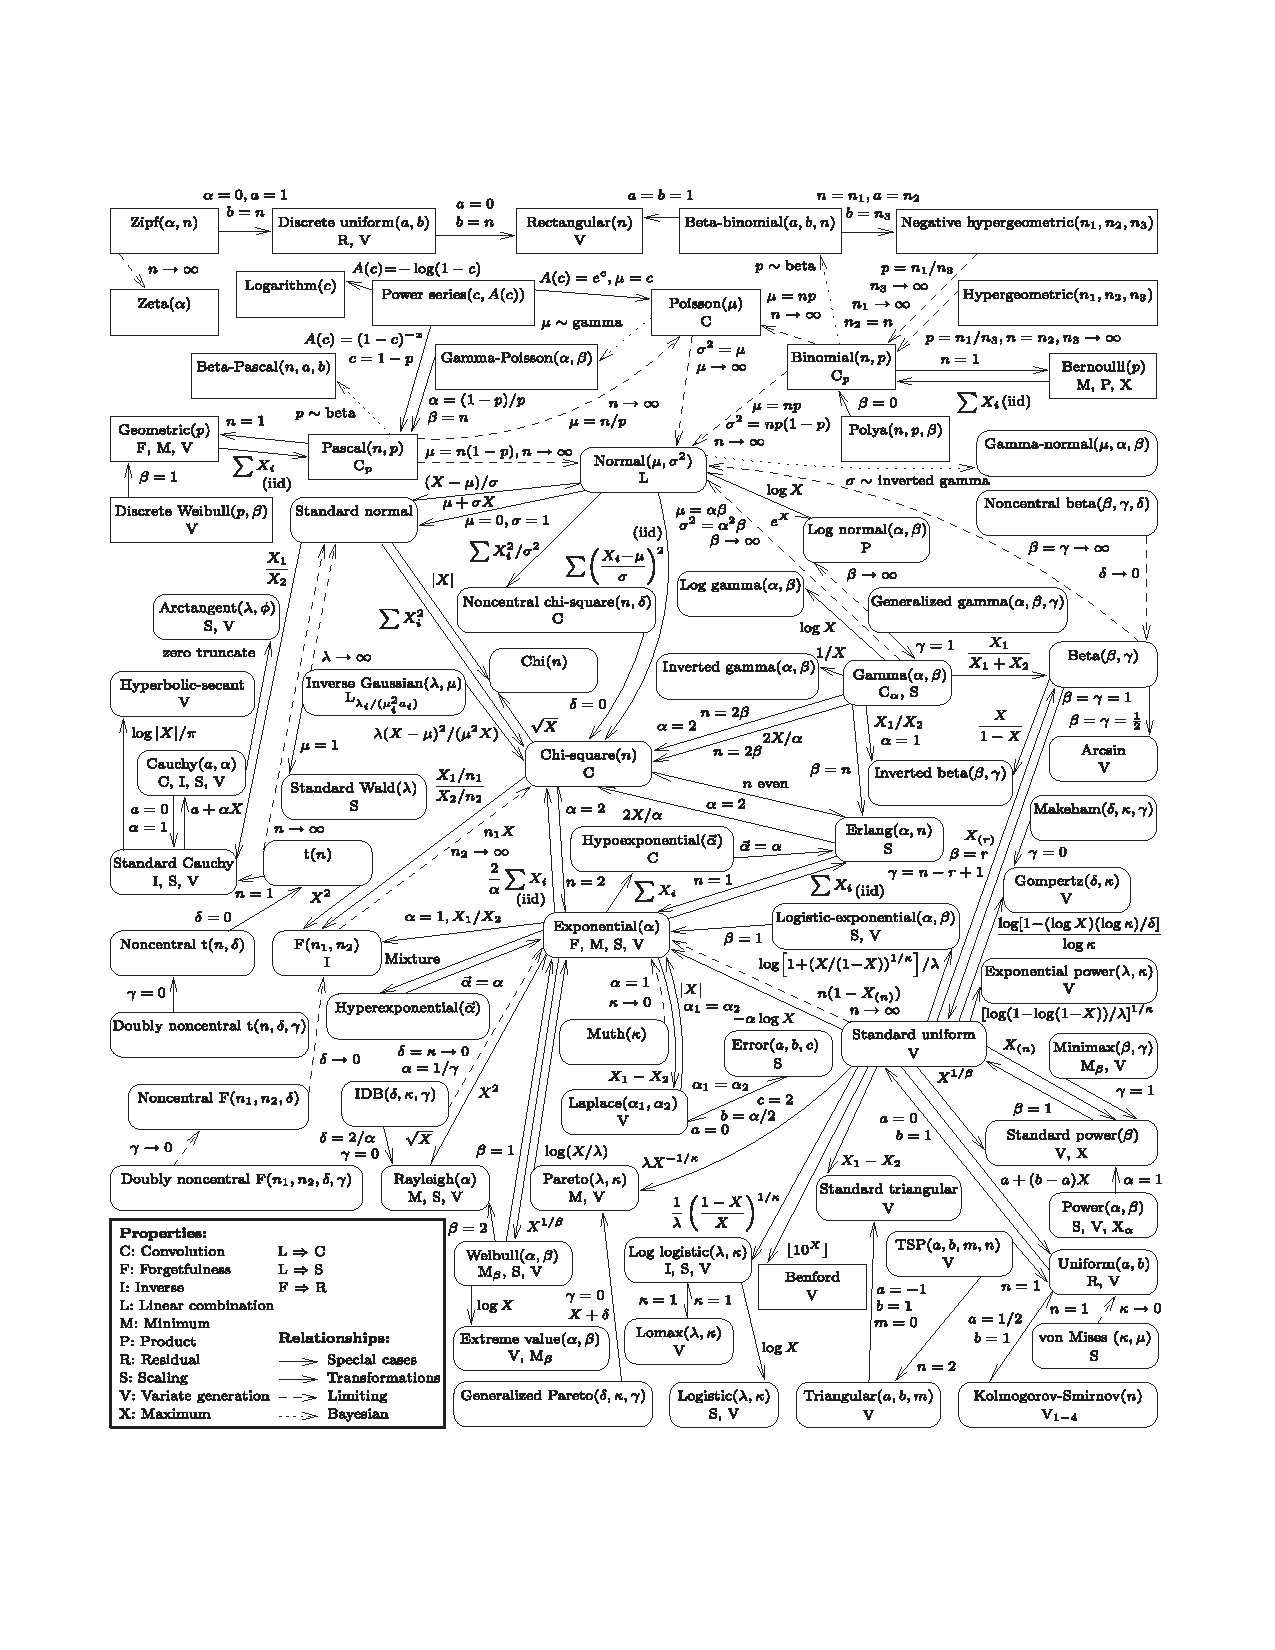
\includegraphics[width=\textwidth]{figs/relationships}
  \caption{\T{Univariate distribution relationships,
  courtesy Leemis and McQueston}~\cite{Leemis08}.}
\end{sidewaysfigure}

\end{document}
